% This must be in the first 5 lines to tell arXiv to use pdfLaTeX, which is strongly recommended.
\pdfoutput=1
% In particular, the hyperref package requires pdfLaTeX in order to break URLs across lines.

\documentclass[11pt]{article}

% Change "review" to "final" to generate the final (sometimes called camera-ready) version.
% Change to "preprint" to generate a non-anonymous version with page numbers.
\usepackage[final]{acl}

% Standard package includes
\usepackage{times}
\usepackage{latexsym}

% For proper rendering and hyphenation of words containing Latin characters (including in bib files)
\usepackage[T1]{fontenc}
% For Vietnamese characters
% \usepackage[T5]{fontenc}
% See https://www.latex-project.org/help/documentation/encguide.pdf for other character sets

% This assumes your files are encoded as UTF8
\usepackage[utf8]{inputenc}

% This is not strictly necessary, and may be commented out,
% but it will improve the layout of the manuscript,
% and will typically save some space.
\usepackage{microtype}

% This is also not strictly necessary, and may be commented out.
% However, it will improve the aesthetics of text in
% the typewriter font.
\usepackage{inconsolata}

%Including images in your LaTeX document requires adding
%additional package(s)
\usepackage{graphicx}

\usepackage{latexsym}
\usepackage{tabularx} % \usepackage{arydshln}
\usepackage{booktabs}
\usepackage{multirow}
\usepackage{subfigure}
\usepackage{amsmath}
\usepackage{amssymb}
\usepackage{array}
\usepackage{bm}
\usepackage{xparse}
\usepackage{mathtools}
\usepackage{pifont}
\usepackage{enumitem}
\usepackage{tcolorbox}
\tcbuselibrary{breakable}
\usepackage{listings}
 
\usepackage{arydshln}
\usepackage{hyperref}

% If the title and author information does not fit in the area allocated, uncomment the following
%
%\setlength\titlebox{<dim>}
%
% and set <dim> to something 5cm or larger.

\title{Evaluating Personalized Tool-Augmented LLMs from the Perspectives of \\ Personalization and Proactivity}

% Author information can be set in various styles:
% For several authors from the same institution:
% \author{Author 1 \and ... \and Author n \\
%         Address line \\ ... \\ Address line}
% if the names do not fit well on one line use
%         Author 1 \\ {\bf Author 2} \\ ... \\ {\bf Author n} \\
% For authors from different institutions:
% \author{Author 1 \\ Address line \\  ... \\ Address line
%         \And  ... \And
%         Author n \\ Address line \\ ... \\ Address line}
% To start a separate ``row'' of authors use \AND, as in
% \author{Author 1 \\ Address line \\  ... \\ Address line
%         \AND
%         Author 2 \\ Address line \\ ... \\ Address line \And
%         Author 3 \\ Address line \\ ... \\ Address line}

% \author{First Author \\
%   Affiliation / Address line 1 \\
%   Affiliation / Address line 2 \\
%   Affiliation / Address line 3 \\
%   \texttt{email@domain} \\\And
%   Second Author \\
%   Affiliation / Address line 1 \\
%   Affiliation / Address line 2 \\
%   Affiliation / Address line 3 \\
%   \texttt{email@domain} \\}


\author{
 \textbf{Yupu Hao\textsuperscript{1,2}},
 \textbf{Pengfei Cao\textsuperscript{1,2}},
 \textbf{Zhuoran Jin\textsuperscript{1,2}},
 \textbf{Huanxuan Liao\textsuperscript{1,2}},
\\
 \textbf{Yubo Chen\textsuperscript{1,2}},
 \textbf{Kang Liu\textsuperscript{1,2}},
 \textbf{Jun Zhao\textsuperscript{1,2}},
\\
 \textsuperscript{1}The Key Laboratory of Cognition and Decision Intelligence for Complex Systems, \\Institute of Automation, Chinese Academy of Sciences, Beijing, China\\
 \textsuperscript{2}School of Artificial Intelligence, University of Chinese Academy of Sciences, Beijing, China
\\
\{haoyupu2023, liaohuanxuan2023\}@ia.ac.cn, \\ \{pengfei.cao, zhuoran.jin, yubo.chen, kliu, jzhao\}@nlpr.ia.ac.cn
 % \small{
 %   \textbf{Correspondence:} \href{mailto:email@domain}{email@domain}
 % }
}

\begin{document}
\maketitle
\begin{abstract}
Personalized tool utilization is essential for aligning large language models (LLMs) with user preference in interaction scenarios with various tools. However, most of the current benchmarks primarily focus on either personalization of text generation or direct tool-utilizing, without considering both. In this work, we introduce a novel benchmark \textbf{ETAPP} for evaluating personalized tool invocation, establishing a sandbox environment, and a comprehensive dataset of 800 testing cases covering diverse user profiles. To improve the accuracy of our evaluation, we propose a key-point-based LLM evaluation method, mitigating biases in the LLM-as-a-judge system by manually annotating key points for each test case and providing them to LLM as the reference. Additionally, we evaluate the excellent LLMs and provide an in-depth analysis. Furthermore, we investigate the impact of different tool-invoking strategies on LLMs' personalization performance and the effects of fine-tuning in our task. The effectiveness of our preference-setting and key-point-based evaluation method is also validated. Our findings offer insights into improving personalized LLM agents. Our Code is available at \url{https://github.com/hypasd-art/ETAPP}.


\end{abstract}

\section{Introduction}
With the advancement of large language model (LLM) capabilities \cite{zhao2024surveylargelanguagemodels}, more researchers are shifting their alignment objectives from targeting the general human population to focusing on specific small groups or individuals \cite{chen2024personapersonalizationsurveyroleplaying, jang2023personalized}. Personalizing the LLMs refers to adjusting the behavior and output of LLMs to match the needs of individual users better. In this context, \citeauthor{li2024personalllmagentsinsights}\shortcite{li2024personalllmagentsinsights} introduce the concept of the \textit{Personal LLM Agents}, which integrates personalized user data and devices to provide user with comprehensive, continuous, and personalized service. To achieve this goal, the Personal LLM Agents must possess two key capabilities: memory \cite{zhang2024surveymemorymechanismlarge} and interaction \cite{10.1145/3704435, mialon2023augmentedlanguagemodelssurvey}. The memory capability allows the model to track and retain both the user's current state and their historical information, enabling more personalized and context-aware interactions. Meanwhile, the interaction capability empowers the model to engage with external systems and devices, utilizing tools to perform tasks and support the user’s needs in real-time \cite{li-etal-2023-api, DBLP:conf/iclr/QinLYZYLLCTQZHT24}.




Currently, Personal LLM Agent evaluations mainly focus on text generation \cite{zhao2025do}, with limited attention to external interactions. Only a few recent studies have begun to assess Personal LLM Agents in interactive scenarios involving tool utilization. For example, \citeauthor{wang2024aipersonalifelongpersonalization}\shortcite{wang2024aipersonalifelongpersonalization} constructs a life-long personal agent framework and evaluates it using LLM. Although their work incorporates tool calling by simulating the external API execution, it does not conduct a specialized evaluation of the interaction process itself. \citeauthor{cai2024largelanguagemodelsempowered}\shortcite{cai2024largelanguagemodelsempowered} evaluates personalized tool usage in the specific domain of online shopping with a limited set of tools. However, these works still fail to answer the following core questions: (1) Compared to normal tool-utilizing, what evaluation metrics should be designed to assess personalized tool-utilizing? (2) How can we effectively evaluate the personalized tool usage capability in more realistic environments, beyond the narrow domain and the simulated scenarios?





\begin{figure*}[t]
  \centering
  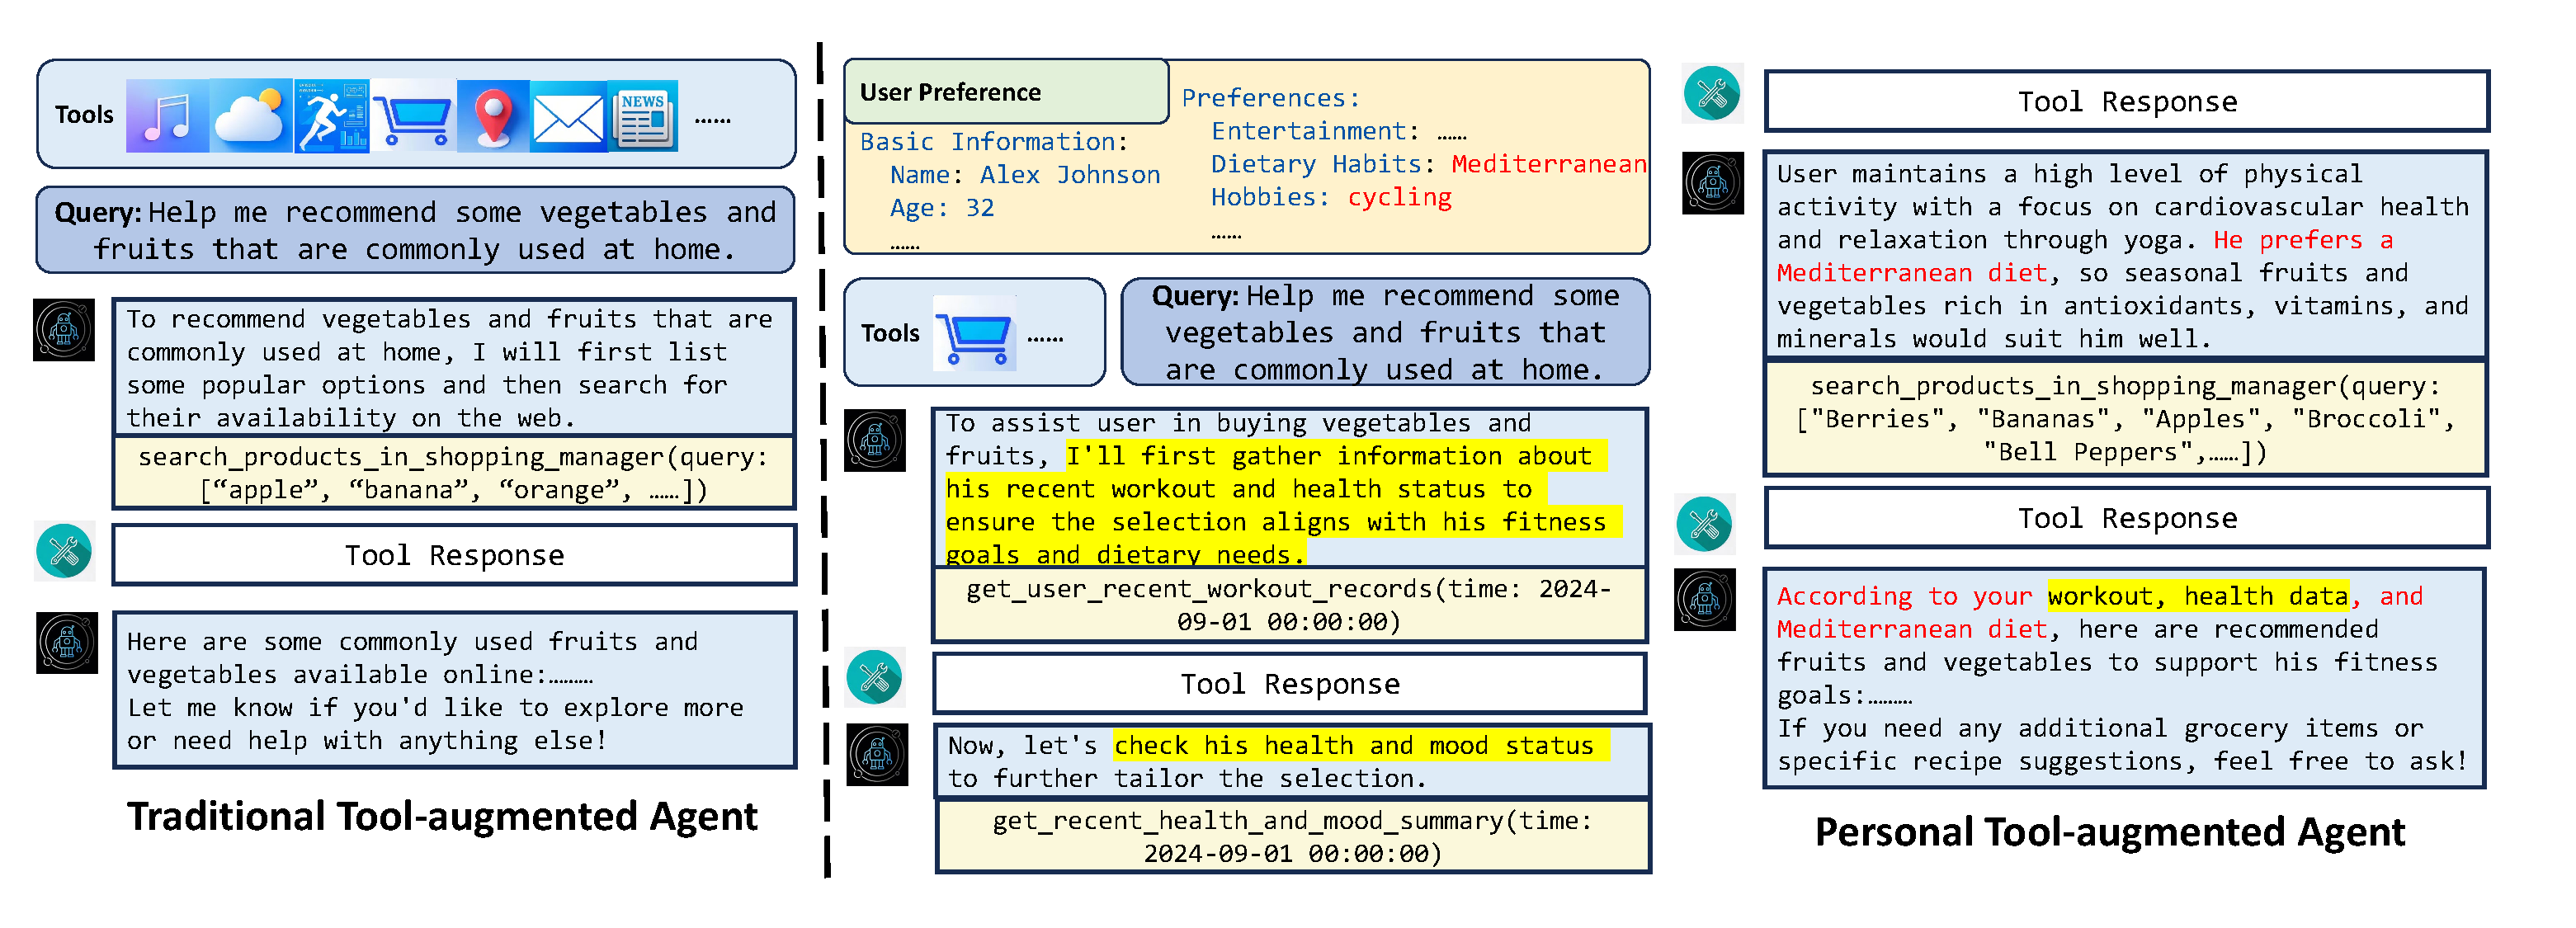
\includegraphics[width=0.95\textwidth]{pic/different_model.pdf} 
  \caption{The difference between a traditional tool-augmented agent and a personal tool-augmented agent. Red font represents output reflecting personalization, while yellow background font represents output reflecting proactivity.
  }
    \label{fig:different_model}
\end{figure*}

To answer the first question, we argue that an ideal personal assistant should not only provide personalized services but also understand the user's intentions and anticipate unspoken needs. It should offer comprehensive support by considering factors beyond immediate instructions, easing the user's burden. From this perspective, Figure~\ref{fig:different_model} illustrates the distinctions between traditional tool-augmented LLMs and personal tool-augmented LLMs. The latter should exhibit two key features: personalization and proactivity. \textbf{Personalization} ensures the model tailors its responses and tool usage based on the user's preferences and needs. For example, when the user asks for food recommendations, the personalized LLM considers that the user prefers a Mediterranean diet (highlighted in red font), in contrast to traditional agents that offer popular options. \textbf{Proactivity} refers to the model anticipating and suggesting actions beyond the user's request to help complete tasks more comprehensively. For instance, the assistant checks the user's recent health status and workout records to further tailor the recommendation (highlighted in yellow background), unlike traditional models, which overlook these factors. This action is not required by the user but effectively enhances the quality of services. 







Based on the two metrics mentioned above, we construct a new benchmark called \textbf{E}valuation of \textbf{T}ool-augmented \textbf{A}gent from the \textbf{P}ersonalization and \textbf{P}roactivity Perspective (\textbf{ETAPP}) to evaluate the personalized tool invocation capabilities of large language models. For the tool-invoking framework, we build a simple sandbox to ensure the stability of the testing process, comprising the following key elements: (1) Environment Setup: We develop a tool-invoking system with 33 functional APIs (e.g., \textit{add\_calendar}, \textit{view\_calendar}, \textit{get\_weather}) belonging to 9 categories (e.g., \textit{Calendar}, \textit{Weather}), including software APIs and hardware APIs. To enhance the authenticity and stability of the evaluation, we design a simple sandbox environment where the API responses are not influenced by external environmental changes. (2)	Memory Building: The memory of personal LLM agents includes long-term user preferences and short-term user status. We divide user preferences into two categories: high-level user profiles and low-level tool-utilizing preferences, which help us to capture user needs more precisely. We generate 16 different user profiles based on professional backgrounds, which serve as the foundation for generating diverse evaluation samples. To simulate real usage scenarios, we construct 9 days of interaction history for each necessary tool and user.
(3)	Instruction Construction: We manually label 50 test instructions, and combine them with 16 different user profiles to create a final dataset of 800 testing cases. This data supports our evaluation of personalized tool invocation capabilities from two perspectives: personalization and proactivity. 




To address the second question, we use LLM as the evaluating model to score the performance of the tool-invoking system \cite{li2025generationjudgmentopportunitieschallenges, li2024llmsasjudgescomprehensivesurveyllmbased}. To improve the evaluation reliability, we design a key-point-based LLM evaluation method. Each testing instruction is associated with several key points annotated by humans, which serve as standard indicators for task completion. These key points are provided to the evaluation LLM to assist in scoring. The evaluation model first analyzes whether each point is satisfied and provides final analysis and score. Experimental results demonstrate that these key points significantly enhance the evaluation accuracy. 






Finally, we evaluate current excellent LLMs with tool invocation capabilities on the entire set and some reasoning models (e.g., o1-mini, DeepSeek-R1) on a testing subset. The results may suggest that LLMs tend to answer the question directly without deeply reasoning why choosing this tool or have insufficient consideration of the personalized tool-utilizing process. Furthermore, we analyze the impact of different tool-invoking methods on the performance and the results point out the importance of the reasoning process in tool-utilizing. Additionally, we manually label a portion of the testing data and fine-tune a 7B model using these data. The results show that fine-tuning improve performance on in-domain instruction data but has limited effect on out-of-domain instruction data. 






To summary, the contribution of our work includes:
\begin{itemize}
    \item We develop a new benchmark for personalized tool invocation and establish a stable and consistent sandbox environment for evaluation. Using a dataset of 800 test cases with various user profiles and preferences, we evaluate the model's performances from both personalization and proactivity perspectives.
    \item We propose a key-point-based LLM evaluation method utilizing manually annotated key points to assist the evaluation for each testing data, improving the reliability compared with directly evaluating. 
    \item We specifically evaluate the effectiveness of our preference design and evaluation methods. We analyze the impact of different tool-invoking methods and conduct an in-depth analysis of how fine-tuning affects model performance in different scenarios.
\end{itemize}





\section{Dataset Construction}
As shown in Figure~\ref{fig:process_construction_dataset}, this process includes the following components: Environment Setup, Memory Building, and Instruction Construction.



\subsection{Environment Setup}
To better simulate real-world application scenarios, we manually construct a tool-invoking environment comprising 33 functional APIs (e.g., \textit{add\_calendar}, \textit{get\_weather}) belonging to 9 categories and 2 tool retrieval APIs (\textit{search\_tools} and \textit{get\_tool\_doc}) to search for usable tools. These APIs encompass a wide range of common software APIs (e.g. Calendar and Email) and hardware-dependent APIs (e.g. health monitoring through smart wristbands and smart home control), ensuring a broad range of practical use cases.



Additionally, we develop a simple sandbox environment to ensure the stability and reliability of the testing process. This sandbox isolates the experiment from external environmental variables (e.g., connection error or change of world), thereby preventing any external factors from influencing the API outputs and ensuring the accuracy of the evaluations. Real-world API data is used to generate corresponding outputs (e.g., data from RapidAPI), enhancing the authenticity of the simulated scenarios. For further details, please refer to Appendix~\ref{sec:dataset_construction}.




\begin{figure}[t]
  \centering
  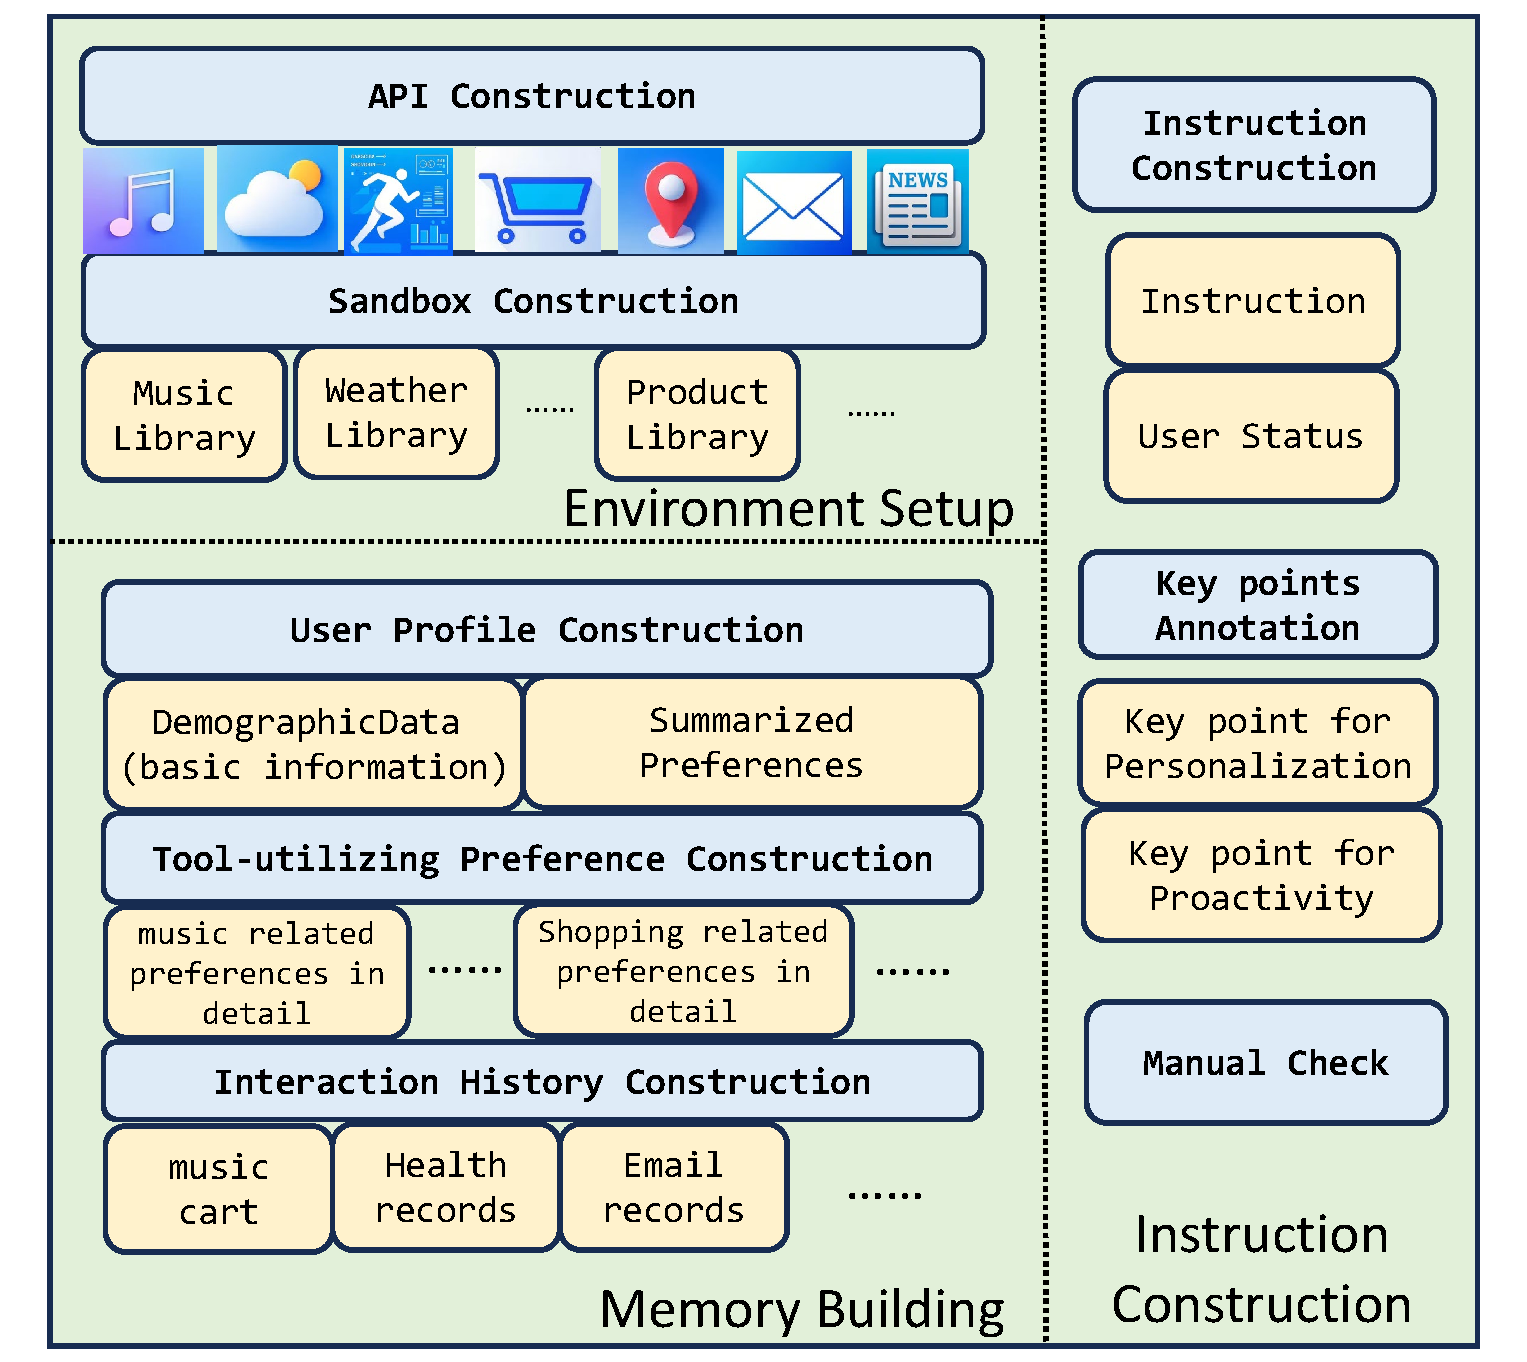
\includegraphics[width=\columnwidth]{pic/construct_dataset.pdf} 
  \caption{The process of dataset construction.
  }
    \label{fig:process_construction_dataset}
\end{figure}





\subsection{Memory Building}
The core of personalization of LLM lies in effectively utilizing the memory of the user, which can be divided into long-term memory (capturing the user's preferences, habits, and historical behaviors) and short-term memory (reflecting the user's current state like position). % and 

\subsubsection{Long-term and Short-term Memory}
For long-term memory, we propose a novel architecture by subdividing user preferences into two categories to manage the memory more effectively: \textbf{high-level preferences} (User Profile) and \textbf{low-level preferences} (Tool-utilizing Preference). 
The User Profile includes basic information about the user (such as name, age, and occupation) and a summary description of their preferences, while the Tool-utilizing Preference includes a detailed description of the user's preferences for the API in the corresponding category. For example, for APIs related to the music category, we have established a unified music-utilizing preference, which includes attributes such as favorite music, singer, listening habits, etc., providing more detailed guidance for the model to invoke corresponding tool and generate responses. We establish eight types of tool-utilizing preferences for each user (with no preferences designed for the \textit{Weather} category). When a corresponding tool is invoked, the relevant category of preference is input into the model in advance, serving as contextual information to assist the model in generating personalized outputs.

Inputting all preferences at once is neither practical nor efficient due to the vast amount of user data and context window limitations. Traditional methods \cite{zhao2025do}, which summarize preferences from dialogue history, often result in sparse and incomplete coverage, with some preferences not even being reflected in conversations. In contrast, summarizing preferences through API perspective is more comprehensive and accurate.



In detail, we conduct the following memory construction process with the help of LLM. First, the LLM generates 16 different user profiles based on various professions. These profiles are manually verified for diversity and consistency to ensure they cover a wide range of user types. Secondly, based on the above profile, the LLM further generates 8 tool-utilizing preferences for each user, which are then manually verified to ensure relevance and accuracy.


For short-term memory, we define the user's current state for each testing data, including location and current time, reflecting the user's personalized needs more accurately.


\subsubsection{Interaction History Construction}
It is essential to note that some tools rely on the user's interaction history (e.g., retrieving recent exercises or email records). So we need to construct the interaction history for specific APIs. 

To ensure the consistency of the interaction history, we first build a 9-day arrangement for each user and construct an interaction history based on it, covering schedule arrangements, alarms, health status (updated hourly), exercise records, email records, and music collections. The specific steps are in Appendix~\ref{sec:appendix_instruction_history}. 








\subsection{Instruction Construction}
\label{sec:instruction_construction}
We manually label 50 unique instructions, combining them with 16 predefined user profiles to create a total of 800 testing instructions. For each instruction, we provid the user status (current time and location of the user). To ensure the accuracy of the interaction history and avoid potential conflicts, we further verify the 9-day interaction history again to ensure every instruction can get an answer. In addition, we manually write the key points for each instruction. We define these key points as the specific requirements that need to be met within our predefined environment to achieve personalization and proactivity. These key points are used for the evaluation in Section~\ref{sec:evaluation_framework}. For statistics of our dataset, please refer to Table~\ref{table:statistics}.





\begin{figure*}[t]
  \centering
  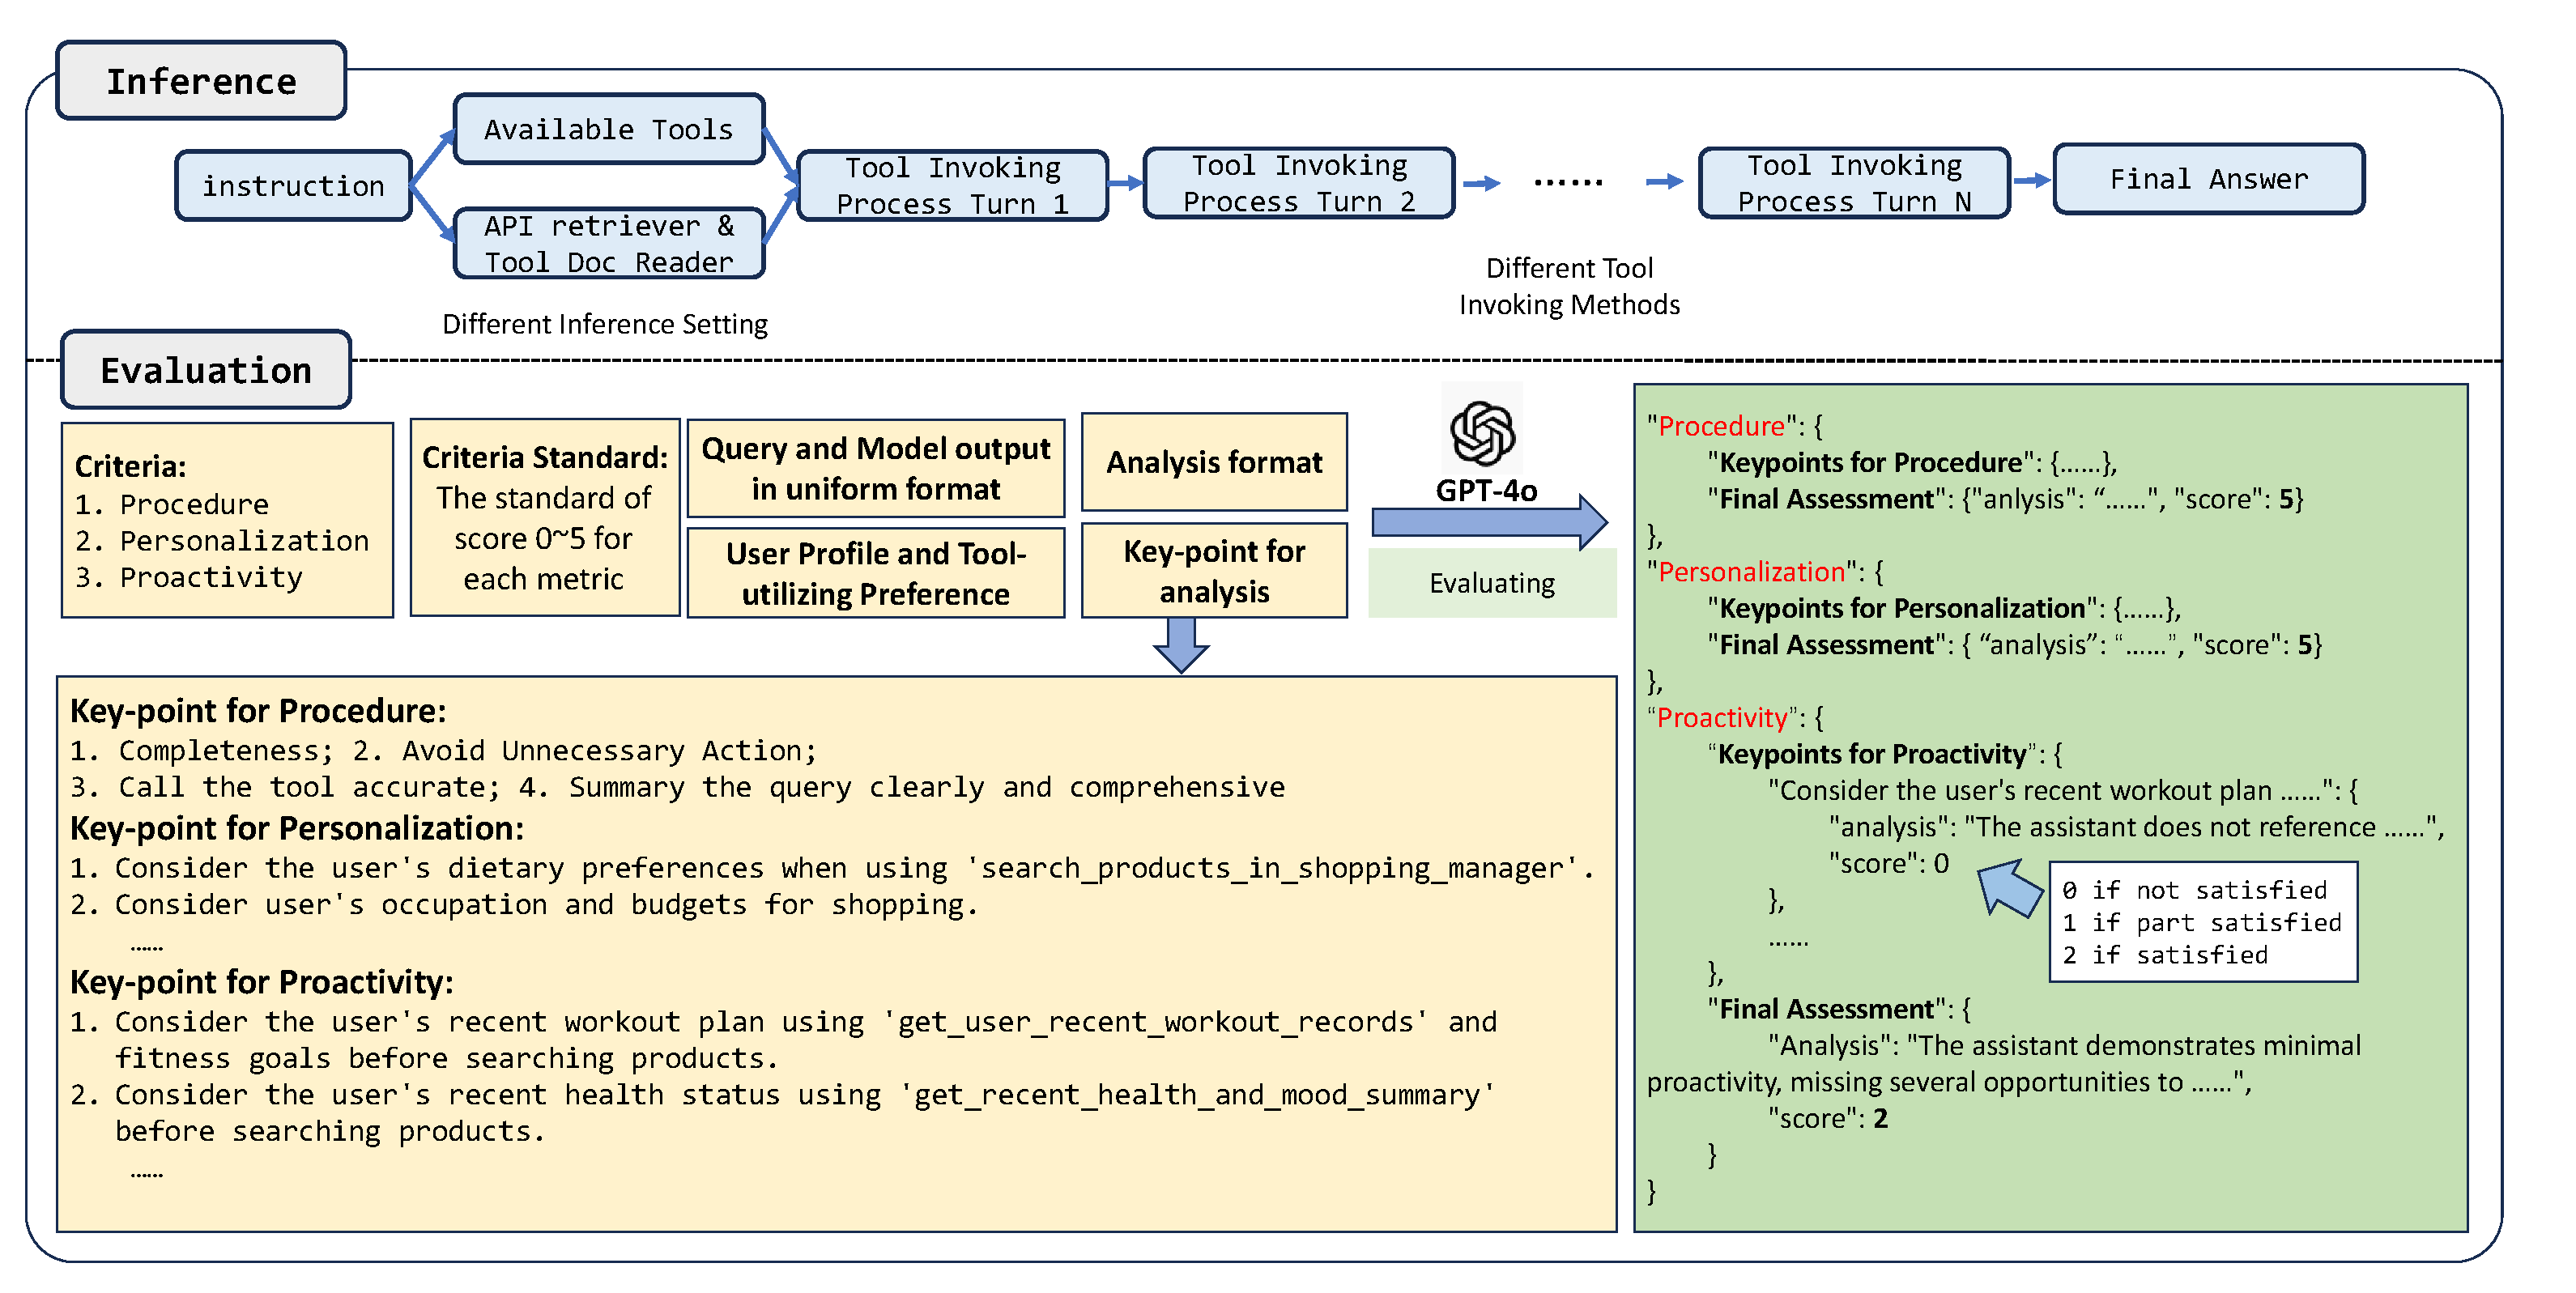
\includegraphics[width=\textwidth]{pic/model_arc.pdf} 
  \caption{The process of Inference and Evaluation of our benchmark.
  }
    \label{fig:process}
\end{figure*}
\section{Evaluation}
\subsection{Evaluation Metrics}
The evaluation process employs a large language model for scoring, with criteria based on three dimensions, each rated on a scale of 0 to 5:
(1)	\textbf{Procedure (PRC)}: This metric assesses whether the model provides a complete and accurate final response. The scoring criteria are based on whether the model addresses all key aspects of the user's query and delivers a clear, comprehensive solution without omissions.
(2)	\textbf{Personalization (PSN)}: This metric evaluates whether the model appropriately incorporates the user's preferences and current status into its response, tailoring its solution to the user’s historical data and requirements.
(3)	\textbf{Proactivity (PTV)}: This metric measures whether the model exceeds the user’s explicit instructions by taking additional, meaningful steps to assist the user effectively, proactively identifying user needs and offering extra suggestions or actions, rather than merely reacting to the user’s request.






\subsection{Evaluation Settings}
The evaluation involves two evaluation settings:
(1)	\textbf{Tool-Given}: In this setting, the tools are pre-specified, and the evaluation focuses on the model’s ability to complete the task effectively with known tools.
(2)	\textbf{Tool-Retrieval}: This setting mirrors real-world scenarios, where the model operates within a limited context window, searching for tools with their corresponding utilizing preferences based on task requirements and invoking them to accomplish the tasks.


Based on the data and methods mentioned above, we construct a complete Inference framework as illustrated in the Figure~\ref{fig:process}. The framework consists of the following components: for user $u$ and instructions $Q$, system prompt $I$, available tools $T_Q$, user preferences of the high-level profile $P_h^u$, user tool-utilizing preferences $\{P_t^u|t \in T_Q\}$, user state $C_Q^u$, one-shot example (optional) $E$. These elements are provided as input to the model, which outputs either a tool invocation or a final response. The LLM processes the instruction by interacting with tools, terminating once the final result is obtained or after reaching a predefined maximum step.




In the Tool-Given and Tool-Retrieval setting, the process is formalized as follows respectively:



\begin{equation}
\footnotesize
\begin{aligned}
    A_n&:\text{Tool\_Given} = LLM(I, T_Q^u, P_h^u, \{P_t^u|t \in T_Q\}, \\ &C_Q^u, E, Q, \sum_{i=1}^{n-1}(A_i, O_i))\\
    A_n&:\text{Tool\_Retrieval} = LLM(I, T_Q^u, P_h^u, C_Q^u, E, Q, \\ &\sum_{i=1}^{n-1}(A_i, O_i, \{P_t^u|t \in o_i^j \And a_i^j=\text{tool\_search}\}))
\end{aligned}
\end{equation}


where, an step $i$, $A_i$ is the output of LLM, $a_i^j$ is the j-th tool calling in $A_i$, $O_i$ represents the observation of corresponding tool.







\subsection{Evaluation Framework}
\label{sec:evaluation_framework}
We propose the key-point-based LLM evaluation framework. Due to the non uniqueness of the solution path and the multi-dimensionality and difficulty of preference evaluation, common methods generally use LLMs as evaluators in evaluating tool utilizing ability \cite{DBLP:conf/iclr/QinLYZYLLCTQZHT24} or preference alignment \cite{zhao2025do}. However, we find that directly evaluating LLM performance is difficult because the evaluation model has limited understanding of personalization and proactivity and cannot easily judge whether the output meets the required standards. To improve this, we need to encourage the evaluation model $E\_LLM$ to analyze the model's output through concrete aspects, so we provide the key points written manually to the evaluation LLM. 






As shown in Figure~\ref{fig:process}, for each instruction $Q$ and user $u$, the criteria standard of the score from 0 $\sim$ 5 is provided in system prompt $I_E$. The user profile preference and tool-utilizing preferences, and the output of the model is provided to the evaluation model. Besides, the key points for each metric $K$ and the analysis format of the output $F$ are provided. The evaluation model outputs the analysis and score (0 $\sim$ 2) for each key point and gives the final score for the model's performance of instruction. The formula is as follows:


\begin{equation}
\footnotesize
\begin{aligned}
    & \text{Analysis}, \text{Score} = E\_LLM(Q, I_E, P_h^u, \\ &\{P_t^u|t \in T_Q\}, \sum_{i=1}^{N}(A_i, O_i), K, F)
\end{aligned}
\end{equation}






\begin{table*}[t]
\centering
{
    
	\centering
    \resizebox{1\textwidth}{!}{
	\begin{tabular}{l | c | c c c | c  c  c | c } %
        \hline
		% \toprule
        
        
        \multirow{2}{*}{\textbf{Model}} 
        & \multirow{2}{*}{\textbf{Method}}
        & \multicolumn{3}{c|}{\textbf{Tool Given}}
        & \multicolumn{3}{c|}{\textbf{Tool Retrieval}}
        & \multirow{2}{*}{\textbf{Average}}
        \\

		
		&
		& \textbf{PRC}
		& \textbf{PSN}
        & \textbf{PTV}
        & \textbf{PRC}
		& \textbf{PSN}
        & \textbf{PTV}
        &
        \\
		\midrule
        
        
        GPT-4o
        & \multirow{5}{*}{\textbf{FC}}
		& \textbf{3.95} 
		& \textbf{3.37} 
        & \textbf{1.61}
        & 2.67
        & 2.19
        & \textbf{1.08}
        & \textbf{2.48}
        
		\\
        % \cline{1-1}
        % \cline{3-9}
        % \midrule
  
		DeepSeek-V3
        &
		& 3.02 
        & 2.78 
        & 1.47
        & 2.57
        & \textbf{2.38}
        & 0.95 
        & 2.20

        \\
        % \cline{1-1}
        % \cline{3-9}
        % \midrule

        
        Llama-3.1-70B-Instruct
        &
		& 2.31 
        & 1.71 
        & 0.55
        & 1.50
        & 1.06
        & 0.30
        & 1.24

        \\
        % \cline{1-1}
        % \cline{3-9}
        % \midrule


        Qwen2.5-72B-Instruct
        &
		& 3.76 
		& 3.34 
        & 1.5 
        & \textbf{2.72} 
        & 2.31 
        & 1.05
        & 2.45
        
        \\
        % \cline{1-1}
        % \cline{3-9}
        % \midrule
        
        
        watt-tool-70B
        &
		& 2.70 
		& 1.97 
        & 0.71
        & 0.84
        & 0.32
        & 0.12
        & 1.11
        
		\\
        \hline
        \hline
        % \midrule
        % \midrule

        GPT-4o
        & \multirow{7}{*}{\textbf{ReAct}}
		& 3.97 
		& 3.61 
        & 1.60
        & 3.70
        & 3.43
        & 1.56
        & 2.98
        
		\\
        % \cline{1-1}
        % \cline{3-9}
        % \midrule
  
		DeepSeek-V3
        &
		& \textbf{4.05} 
        & \textbf{3.78}
        & 1.84
        & \textbf{3.82}
        & \textbf{3.54}
        & \textbf{1.65} 
        & \textbf{3.11}

        \\
        % \cline{1-1}
        % \cline{3-9}
        % \midrule

        o1-preview *
        &
		& 3.67 
		& 3.69 
        & \textbf{1.87}
        & 3.28
        & 3.48
        & 1.60
        & 2.93
        
		\\
        % \cline{1-1}
        % \cline{3-9}
        % \midrule
  
		o1-mini *
        &
		& 3.63 
        & 3.35 
        & 1.61
        & 3.25
        & 3.14
        & 1.35 
        & 2.72

        \\
        % \cline{1-1}
        % \cline{3-9}
        % \midrule

        
        DeepSeek-R1 *
        &
		& 2.41 
        & 2.06 
        & 1.35
        & 0.93
        & 0.40
        & 0.31
        & 1.24

        \\
        % \cline{1-1}
        % \cline{3-9}
        % \midrule


        DeepSeek-R1-Distill-Qwen-32B *
        &
		& 2.40 
		& 2.57 
        & 1.07 
        & 1.74 
        & 1.66 
        & 0.62
        & 1.68
        
        \\
        % \cline{1-1}
        % \cline{3-9}
        % \midrule
        
        
        QwQ-32B-Preview *
        &
		& 1.01 
		& 1.19 
        & 0.53
        & 0.61
        & 0.48
        & 0.18
        & 0.67
        
		\\
        \hline
        % \midrule



		% \bottomrule
	\end{tabular}
}
}
	\caption{The overall results of different LLMs under two settings. * represents testing on a subset of data. The evaluation model we used is GPT-4o.
	}
	\label{table:overall_result}
\end{table*}











\section{Experiments}
\subsection{Baselines}
We adopt two frequently used tool-invoking methods: \textbf{FC (Function Calling)}: After fine-tuning, the model calls the tool through a predefined format; \textbf{ReAct} \cite{yao2023react}: The model combines reasoning with tool invocation, where reasoning guides the model to analyze the current status and decide the appropriate action. The one-shot example is provided to ReAct in this process. 





We use the excellent closed-source and open-source models with the function calling ability as baselines in two experimental settings. 
Additionally, we evaluate the reasoning model on a subset of the 100 testing data due to the budgets factors using ReAct method, as they do not support FC. For further details refer to Appendix~\ref{sec:evaluation_details}.




\subsection{Evaluation Results}
The results are shown in Table~\ref{table:overall_result}, we can find that in FC result: (1) In the Tool-Retrieval scenario, the model's performance is significantly lower than in the Tool-Given scenario, indicating that the model struggles more as the length and difficulty of tool-invoking and planning increases; (2) Currently, in FC setting, GPT-4o performs excellently across multiple metrics, while Qwen2.5-72B-Instruct outperforms DeepSeek-V3, demonstrating its strong performance; (3) Even the best-performing model in BFCL \cite{berkeley-function-calling-leaderboard}, Watt-tool-70B, struggles with this tool-invoking task. This could be due to two reasons: a) Not generalizing. Post-training may hinder its ability to fully grasp personalization and proactivity within the tool-planning process; b) Not deep reasoning. During tool learning, the model tends to directly invoke tools based on explicit instructions, without deep reasoning, leading to difficulties in effectively handling Proactivity scenarios without clear instructions. This inspires us to not only enhance the model's ability to use tools but also to think about why invoking this tool.


The reasoning models do not show an advantage over non-reasoning models in this task, particularly the DeepSeek-Distill and QwQ models, which performed poorly. The reasoning models may not integrate the reasoning process with the tool-invoking process, or may not have deep thinking on Personalization and Proactivity in the specific scenario. Some error examples can be found in the Appendix~\ref{sec:appendix_example_error}.


\begin{figure*}[t]
  \centering
  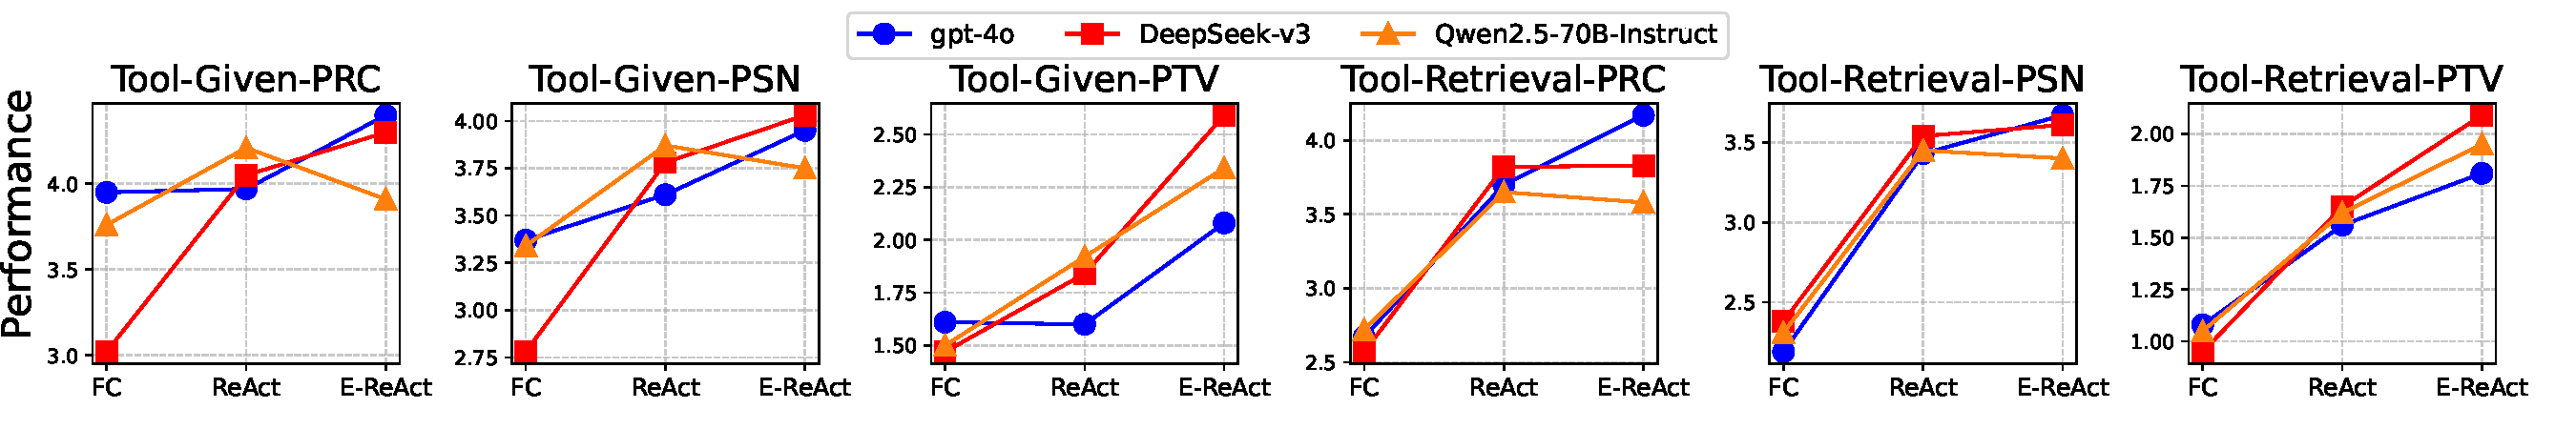
\includegraphics[width=\textwidth]{pic/inference.pdf} 
  \caption{The performance of different tool-invoking methods.
  }
    \label{fig:different_inference_performance}
\end{figure*}

\subsection{Analysis}
\subsubsection{Tool-invoking Method Analysis}
In order to analyze the impact of different tool-invoking methods on model performance, we adopt the following three approaches: \textbf{FC}, \textbf{ReAct} and \textbf{E-ReAct (Enhanced-ReAct)}. The E-ReAct method extends ReAct by first requiring the model to generate key aspects of personalization, proactivity before invoking tools. Once these key points are addressed, the model proceeds with tool invocation using the ReAct framework to complete the task. 




As shown in Figure~\ref{fig:different_inference_performance}, we find that E-ReAct methods can effectively improve the personalization and proactivity capabilities of the model's output. By incorporating a mandatory deep thinking and understanding process before tool invocation, the model better interprets user intentions and provides more proactive services. This suggests that integrating more high-quality reasoning into the tool-learning process may lead to even better performance.



\begin{table}[]
    \centering
    \resizebox{0.9\columnwidth}{!}{
    \begin{tabular}{c|c|c|c|c}
        \midrule
        Setting & Tokens & PRC & PSN & PTV
        \\
        \hline
         All & 3444 &  4.09 & \textbf{3.80}  & 1.62 \\
         \hline
         Needed & \textbf{2393} & \textbf{4.16} & 3.73 & \textbf{1.76}
         \\
         \hline
    \end{tabular}}
    \caption{The results of different preference settings are evaluated on a subset of data. The \textit{Tokens} metric represents the average number of tokens for each instruction calculated by the tokenizer of Llama-3.1-70B-Instruct. And the performance is tested on GPT-4o. 
    }
    
    \label{table:different_preference_setting}
\end{table}
\subsubsection{Preference Setting Analysis}
We divide the preference into the User Profile and Tool-utilizing Preference. Table~\ref{table:different_preference_setting} shows the difference between inputting all preferences into the LLM and our method. We can find that our setting (Needed) reduces the context length and demonstrates competitive results compared to inputting all (All). Notably, we have only included 8 categories of preferences, as the number of categories increases or the preferences become more concrete, the advantage of our setting is expected to become even more prominent. 


\subsubsection{Fine-tuning Experiments Analysis}
To validate our idea of the importance of reasoning, we annotate some data in both ReAct and FC format respectively and conduct fine-tuning experiments on Qwen2.5-7B-Instruct using 200 data points. The annotating process is as follows: 
(1)	Generate reference answers using the LLM.
(2)	Perform manual verification and labeling the answers to ensure quality and consistency.
For data in FC format, one set only includes the tool-calling process, while the other also contains the textual thinking before the tool invocation.

The results are in the Table~\ref{table:fine-tuning-result}. We find that: (1) The performance improves significantly for ID instructions and OOD users. However, with the phenomenon improvement for OOD instructions being significantly lower than for ID instructions, this indicates that for instructions within the same scenario, once the model learns the tool invocation process, it can generalize and solve problems even when user preferences differ. However, when a new scenario emerges, the model struggles to reason effectively about how to solve the problem, resulting in limited improvement. (2) Compared to ReAct and FC models, the improvement for ``wo r'' is not significant, demonstrating that a certain level of reasoning process is necessary to enhance the model's multi-turn tool invocation capability. (3) Tool-invoking methods like ReAct still show advantages in this model compared to FC.



\begin{table}[t]
\centering
% \setlength{\tabcolsep}{2pt}
{
   \renewcommand{\arraystretch}{0.9} 
	\centering
    \resizebox{1\columnwidth}{!}{
	\begin{tabular}{l | c c c } %
		\toprule
        
        
        \textbf{Model} 
        

		
		
		& \textbf{PRC}
		& \textbf{PSN}
        & \textbf{PTV}

        \\
		\midrule

        \multicolumn{4}{c}{\textbf{U(ID)I(OOD)}}
        \\
        \midrule
        \midrule
        
        
        Vanilla (ReACT)
		& 2.76 
		& 2.97 
        & 1.35
        
		\\
        % \midrule
  
		\quad FT (ReAct)
		& \textbf{3.47} ($\uparrow$ 25.8\%) 
        & \textbf{3.28} ($\uparrow$ 10.4\%) 
        & \textbf{1.99} ($\uparrow$ 47.4\%)

        \\
        \midrule
        % \midrule

        
        Vanilla (FC)
		& 3.08 
        & 2.66 
        & 1.07

        \\
        % \midrule


        \quad FT (FC)
		& 3.23 ($\uparrow$ 4.9\%) 
		& 3.00 ($\uparrow$ 12.8\%) 
        & 1.72 ($\uparrow$ 60.7\%) 
        
        \\

        % \midrule
        
        
        \quad FT (FC wo r)
		& 2.67 ($\downarrow$ 13.3\%)
		& 2.68 ($\uparrow$ 0.7\%)
        & 1.62 ($\uparrow$ 51.4\%)
       
		\\
        \midrule

        \multicolumn{4}{c}{\textbf{U(OOD)I(ID)}}
        \\
        \midrule
        \midrule

        Vanilla (ReACT)

        & 3.29
        & 3.28
        & 1.57
        
		\\
        % \midrule
  
		\quad FT (ReAct)
  
        & \textbf{4.09} ($\uparrow$ 24.3\%)
        & \textbf{3.75} ($\uparrow$ 14.3\%)
        & \textbf{2.79} ($\uparrow$ 77.7\%) 

        \\
        \midrule
        % \midrule

        
        Vanilla (FC)
        % Qwen2.5-7B-Instruct (FC)
        & 3.33
        & 2.65
        & 1.07

        \\
        % \midrule


        \quad FT (FC)
 
        & 3.81 ($\uparrow$ 14.4\%) 
        & 3.49 ($\uparrow$ 31.7\%) 
        & 2.37 ($\uparrow$ 121.5\%)
        
        \\

        % \midrule
        
        
        \quad FT (FC wo r)

        & 3.48 ($\uparrow$ 4.5\%)
        & 3.24 ($\uparrow$ 22.3\%)
        & 2.19 ($\uparrow$ 104.6\%)
       
		\\
        \midrule

        \multicolumn{4}{c}{\textbf{U(OOD)I(OOD)}}
        \\
        \midrule
        \midrule




        Vanilla (ReACT)
		
        & 2.91
        & 3.08 
		& 1.43
        
		\\
        % \midrule
  
		\quad FT (ReAct)
		
        & \textbf{3.52} ($\uparrow$ 21.0\%)
        & \textbf{3.43} ($\uparrow$ 11.4\%) 
		& \textbf{2.06} ($\uparrow$ 44.1\%)

        \\
        \midrule
        % \midrule

        
        Vanilla (FC)
		
        & 3.03
        & 2.64 
		& 1.07

        \\
        % \midrule


        \quad FT (FC)
		
        & 3.29 ($\uparrow$ 8.5\%)
        & 3.14 ($\uparrow$ 18.9\%) 
		& 1.73 ($\uparrow$ 61.7\%)
        
        \\

        % \midrule
        
        
        \quad FT (FC wo r)
		
        & 2.73 ($\downarrow$ 9.9\%)
        & 2.77 ($\uparrow$ 4.9\%) 
		& 1.64 ($\uparrow$ 53.3\%)
       
		\\
        \midrule



		% \bottomrule
	\end{tabular}
}
}
	\caption{The results of the Qwen2.5-7B-Instruct model fine-tuned on a subset of instructions. \textbf{U} represents the User, \textbf{I} represents the Instruction. \textbf{ID} indicates the users or instructions are seen in the training data, \textbf{OOD} means not seen in the fine-tuning. ``wo r'' means outputting without reasoning process and directly invoking tools.
	}
	\label{table:fine-tuning-result}
\end{table}

 

\subsection{Effectiveness of key-point-based LLM Evaluation}
\begin{figure*}[htbp]
    \centering
    \begin{minipage}[t]{0.48\textwidth}
        \centering
        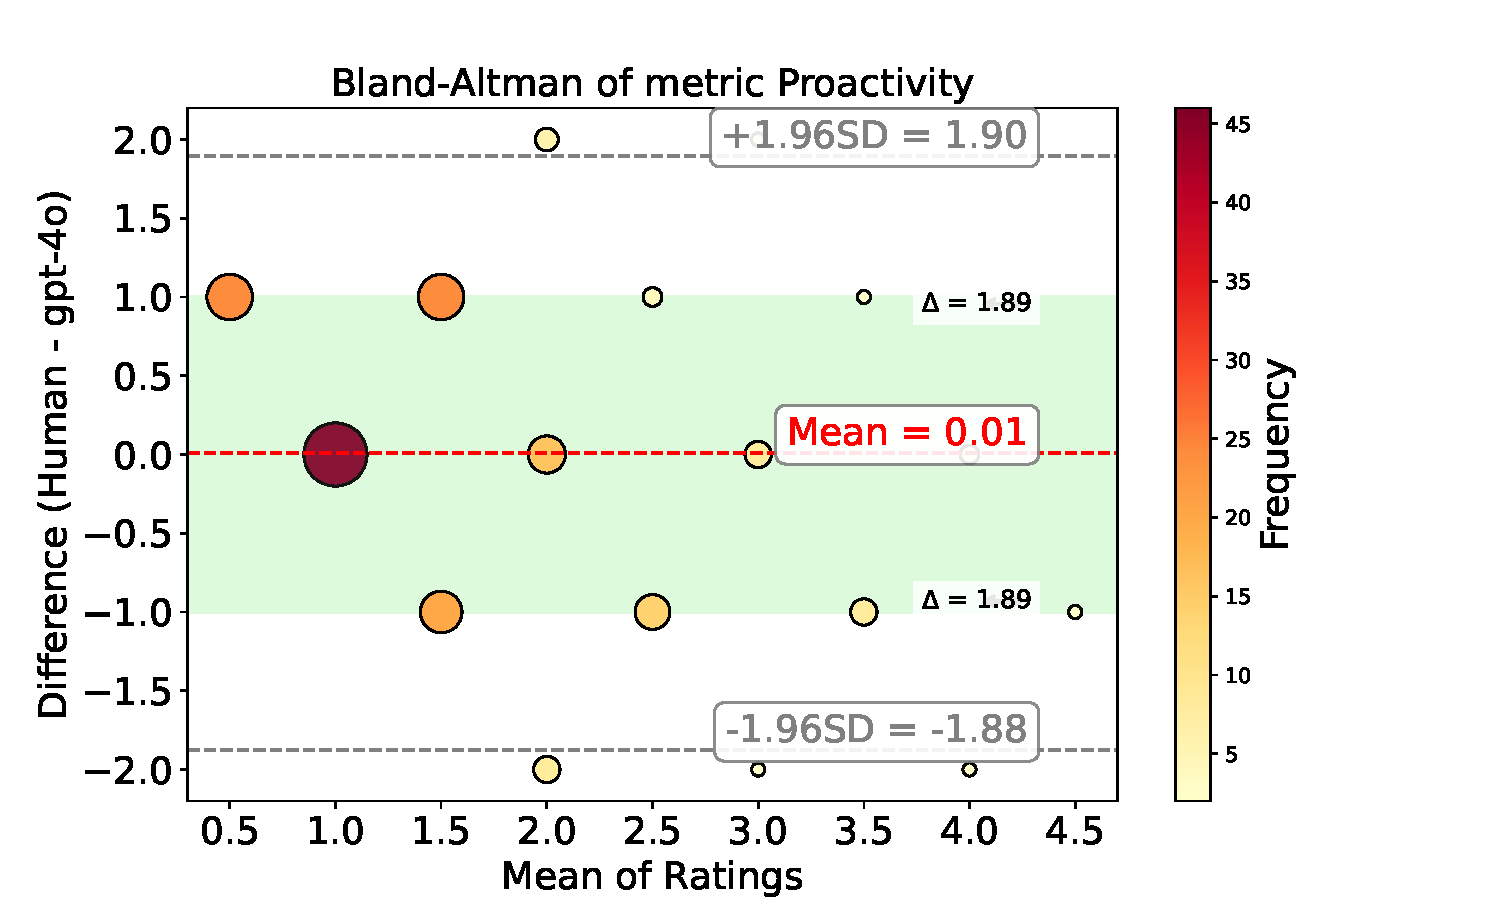
\includegraphics[width=\linewidth]{pic/Proactivity_human_gpt-4o-2024-11-20.pdf}
        \caption{The Bland-Altman analysis result of \textbf{Proactivity} with given key points.}
        \label{fig:w_keypointres_proactivity}
    \end{minipage}
    \hfill 
    \begin{minipage}[t]{0.48\textwidth}
        \centering
        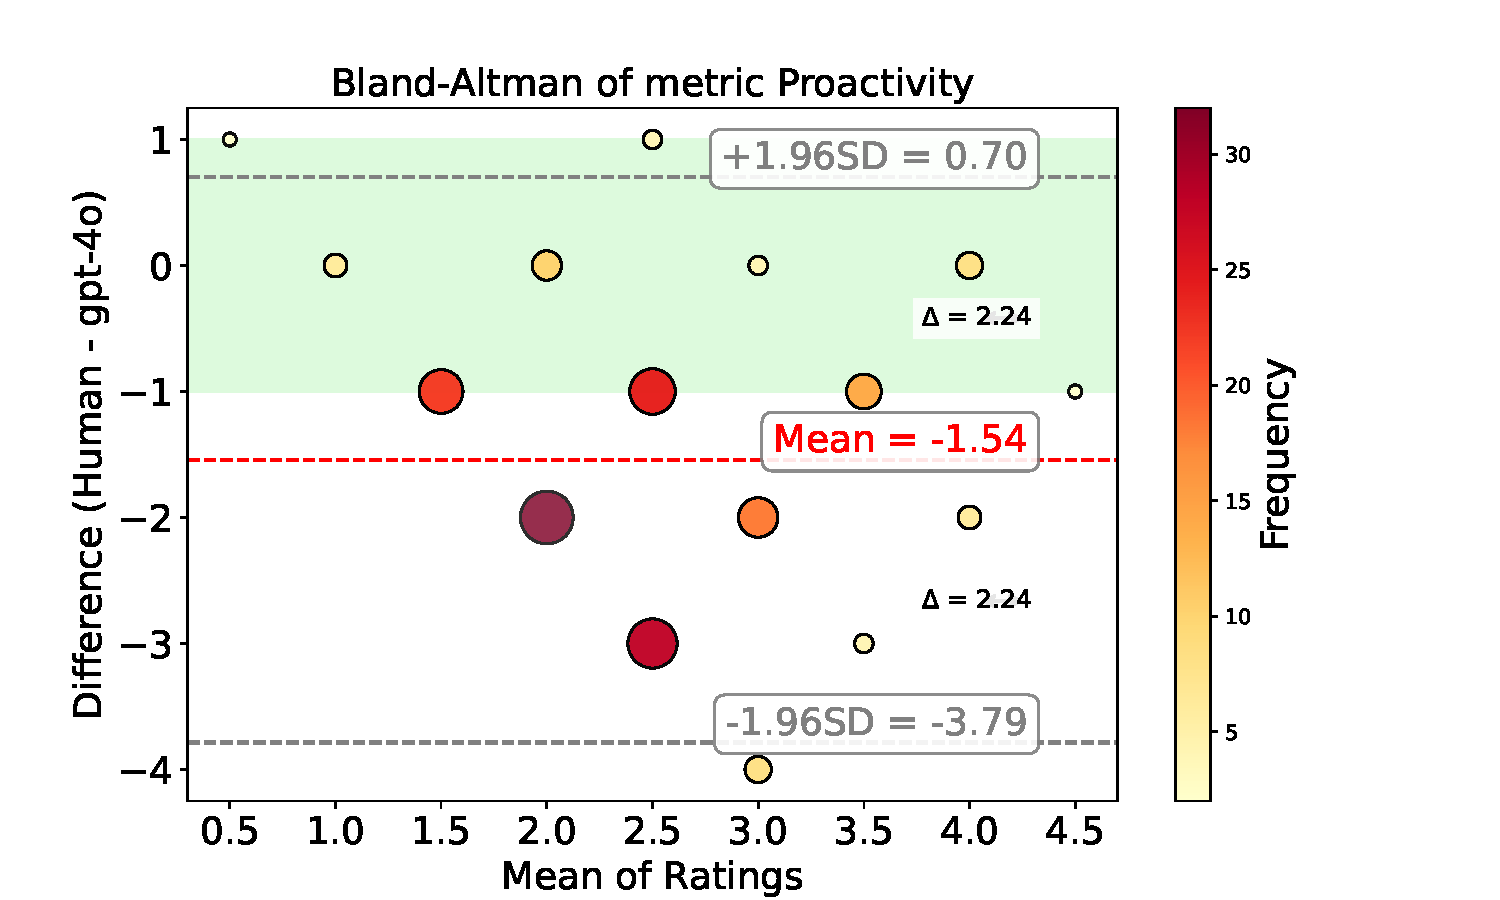
\includegraphics[width=\linewidth]{pic/Proactivity_human_gpt-4o-2024-11-20_wk.pdf}
        \caption{The Bland-Altman analysis result of \textbf{Proactivity} without given key points.}
        \label{fig:wo_keypointres_proactivity}
    \end{minipage}
\end{figure*}



To demonstrate the effectiveness of the key-point-based LLM evaluation method, we collect 16 data points per method in both Tool-Given and Tool-Retrieval settings for model GPT-4o. This result in a total of 96 data points. We then analyze the consistency with human evaluation to validate the method’s effectiveness.
% z





To quantify consistency, we use the Bland-Altman method, which plots the average of two measurements on the x-axis and their difference on the y-axis. Three reference lines are included: the mean difference (red dashed line) and the 95\% limits of agreement (LoA), calculated as mean ± 1.96 × standard deviation. If most of data points fall within the LoA, the methods show good consistency. The point size indicates sample count, and the green area highlights samples with a score difference within 1 point.




The experimental results of metric Proactivity in Figure~\ref{fig:w_keypointres_proactivity} and Figure~\ref{fig:wo_keypointres_proactivity} showed: (1) System Bias Control: Under the key-point constraint, the mean difference is 0.01 (95\% CI: -1.88 $\sim$ 1.90), close to the theoretical ideal value of 0, indicating statistical consistency between LLM and human evaluation in the total score dimension. (2) LoA Interval Length: Compared to the free evaluation mode, the key-point constraint reduces the width of the LoA interval (1.89 vs. 2.24). (3) Error Distribution Characteristics: 89.6\% of the samples show a score difference of $\leq$ 1 point (green area), representing an improvement of over 39.6 percentage points compared to the control group without key points.
These findings confirm the effectiveness of the key-point-based LLM evaluation strategy.
Please refer to Appendix~\ref{sec:appendix_effectiveness_of_key-point-based_LLM_evaluation} for more details.




\section{Related Works}

\subsection{Personalization of LLM}
The personalization of LLMs aims to align with individual preferences \cite{zollo2025personalllm, tseng2024talespersonallmssurvey}. Current personalization tasks are typically focused on specific text generation \cite{he2025cosenhancingpersonalizationmitigating, zhao2025do, lee2024aligningthousandspreferencesmessage}, recommendation tasks \cite{yang2023palrpersonalizationawarellms}, role-playing \cite{wang-etal-2024-rolellm, shao-etal-2023-character}, news headline generation \cite{salemi-etal-2024-lamp}, conversational tasks, as well as applications in education \cite{Pratama2023REVOLUTIONIZINGEH} and healthcare \cite{10.1145/3437963.3441657, abbasian2024conversationalhealthagentspersonalized}, and the evaluation process typically involves summarizing user preferences from the context to generate responses \cite{zhang2024guidedprofilegenerationimproves}. However, the Personal LLM Agents goes further by defining an ideal personal assistant that should possess interactive capabilities \cite{singh-etal-2024-personal}. We propose ETAPP to address the problem that the evaluation of Personal LLM Agents lacks criteria for personalized tool usage in diverse scenarios.  









\subsection{Tool-augmented LLM}
Tool-augmented LLMs aim to enable them to interact with the external world through tools \cite{10.1145/3704435, qu2025tool}. Numerous benchmarks and methods have been proposed to evaluate and improve the accuracy of tool utilization and task completion \cite{trivedi-etal-2024-appworld,li-etal-2023-api, hao2024citienhancingtoolutilizing, tang2023toolalpacageneralizedtoollearning, NEURIPS2023_9cb2a749}. However, these datasets are designed for the general human population rather than for personalized tool invocation tailored to individual user preferences. Our work integrates the tool invocation process with personalization and proposes evaluation metrics and methods for this purpose.




\section{Conclusion}
The paper evaluates the ability and level of large language models to provide personalized services in interactive environments. We integrate the process of tool invocation with personalized services and propose two evaluation metrics: Personalization and Proactivity. To address the unreliability of using LLMs as evaluators in this task, we introduce a key-point-based evaluation method for LLMs and validate its reliability. Finally, we analyze the performance of different models on this task and explore the challenges and potential directions for improving their personalized tool utilization capabilities.

\section*{Limitations}
We evaluate the personalization of tool utilization in LLMs from the perspectives of personalization and proactivity, and propose a key-point-based LLM evaluation method. However, there are still challenges in this area. For example, our work does not consider multimodal tasks. And there are details that can be further refined. For example, during preference modeling, we could further model the selection preferences for similar tools (e.g., when two apps A and B provide the same functionality, users tend to prefer the API from App A to complete the task). In the future, we plan to extend our work to the multimodal domain.

\section*{Ethics Statement}
Our work does not introduce ethical concerns. This paper utilized AI assistance for language polishing of the manuscript, including vocabulary correction and spell checking.


% Bibliography entries for the entire Anthology, followed by custom entries
%\bibliography{anthology,custom}
% Custom bibliography entries only
\bibliography{custom}
\newpage
\appendix


\section{Dataset Construction}
\label{sec:dataset_construction}

\subsection{Tools Construction}
The tools we constructed are in Table~\ref{table:api_name}. Real-world API data are used to generate outputs for most of the tools. For example, the weather data are collected from WeatherAPI.com \footnote{https://rapidapi.com/weatherapi/api/weatherapi-com}, the music data are collected from 
Genius - Song Lyrics \footnote{https://rapidapi.com/Glavier/api/genius-song-lyrics1}  and the shopping products are collected from Real-Time Amazon Data \footnote{https://rapidapi.com/letscrape-6bRBa3QguO5/api/real-time-amazon-data} in RapidAPI. And the Navigation data are modified from TravelPlanner \cite{xie2024travelplanner} which is also collected from Real-World. We change the records' date and add dozens of data points generated by gpt-4o. And the News data are entirely generated by gpt-4o.   

\subsection{The User Preference}
We construct 16 users in our benchmark, each user has a User Profile and Tool-utilizing Preference.

The User Profile example is in Example~\ref{Example:User_Profile}. The example of Tool-utilizing Preference is in Example~\ref{Example:Tool_utilizing_Preference}. One example of the interaction history of API \textit{get\_user\_recent\_workout\_records} of user \textit{James Harrington} is in Example~\ref{Example:Interaction_History}.



\subsection{The Interaction History Construction Process}
\label{sec:appendix_instruction_history}
To ensure the consistency of the interaction history, we first build a 9-day arrangement for each user and construct an interaction history based on it, covering schedule arrangements, alarms, health status (updated hourly), exercise records, email records, and music collections. The specific construction steps for the interaction history are as follows: (1)	Generate the user’s 9-day schedule based on the user profile. (2)	Extend the schedule in detail. (3)	Generate the corresponding interaction history based on the user profile and schedule. (4)	Perform manual verification to ensure consistency and accuracy.

\subsection{Key Points Annotation}
For manually annotated key points, they are annotated and verified by two graduate students to ensure their comprehensiveness and reliability as much as possible.

\section{Evaluation details}
\label{sec:evaluation_details}

\subsection{Tool-invoking Method}
The tool-invoking prompt in FC, ReAct and E-ReAct format in Tool-Given and Tool-Retrieval setting is shown in Prompt~\ref{Prompt:ReAct_Tool_Given}, Prompt~\ref{Prompt:FC_Tool_Given}, Prompt~\ref{Prompt:E-ReAct_Tool_Given}, Prompt~\ref{Prompt:ReAct_Tool_Retrieval}, Prompt~\ref{Prompt:FC_Tool_Retrieval}, Prompt~\ref{Prompt:E-ReAct_Tool_Retrieval}. The item in ``\{'' and ``\}'' will be replaced by specific content in the inference process.





\subsection{Implementation Details}
We use the following model with the function calling ability as baselines in two experimental settings: gpt-4o-2024-11-20, DeepSeek-V3 \cite{deepseekai2024deepseekv3technicalreport}, Qwen2.5-72B-Instruct \cite{qwen2.5}, Llama-3.1-70B-Instruct \footnote{https://huggingface.co/meta-llama/Llama-3.1-70B-Instruct}, and watt-tool-70B \footnote{https://huggingface.co/watt-ai/watt-tool-70B} (the best-performing model in BFCL). 
Additionally, we evaluate the reasoning model o1-preview-2024-09-12, o1-mini-2024-09-12, DeepSeek-R1 \cite{deepseekai2025deepseekr1incentivizingreasoningcapability}, DeepSeek-R1-Distill-Qwen-32B \cite{deepseekai2025deepseekr1incentivizingreasoningcapability}, and QwQ-32B-Preview \cite{qwq-32b-preview} evaluated on a subset of the 100 testing data due to the budgets factors using ReAct method, as they do not support FC. 



For the reasoning model, the reasoning content is not included in the tool-invoking process in our experiments.

For the fine-tuning experiments, we fine-tune the model with LoRA. The rank r is set to 8 and the lora alpha is 16. While the epoch is set to 3 and the learning rate is 1e-4. The batch size is set to 32. The data is in interaction format and we divide each interaction turn with APIs as training data, and we totally divide 200 instructions we annotated into 841 training data. The experiments are conducted on NVIDIA A100.

\subsection{Prompt of Evaluation}
The Prompt of key-point-based LLM Evaluation is in Prompt~\ref{Prompt:Key_Point_Evaluation}. The item in ``\{'' and ``\}'' will be replaced by specific content in the evaluation process. One evaluation output conducted by GPT-4o is shown in Example~\ref{Example:Evaluation_Result_Example}.

\subsection{Example of Error}
\label{sec:appendix_example_error}
Some error examples are shown in Example~\ref{Example:Example_of_Error}.

\section{Effectiveness of key-point-based LLM evaluation}

\label{sec:appendix_effectiveness_of_key-point-based_LLM_evaluation}
The Bland-Altman analysis results of metrics Procedure and Personalization are in Figure~\ref{fig:w_keypointres_procedure}, Figure~\ref{fig:wo_keypoint_res_procedure}, Figure~\ref{fig:w_keypoint_res_personalization}, Figure~\ref{fig:wo_keypoint_res_personalization}. We observe that key points play a crucial role in improving the alignment of the evaluation process for the metrics of Personalization and Proactivity. Although the evaluation model is provided with scoring criteria, it tends to assign higher scores even without the key points. We think this may be because the model lacks sufficient knowledge and understanding of how an assistant can provide personalized and proactive services. Once the key points are input, the evaluation model can analyze whether each point is satisfied, which enhances the final analysis and the accuracy of the score. However, we also notice that the mean difference in the Procedure metric performs worse when key points are included. This may be due to the simultaneous evaluation of all three metrics, where Procedure is influenced by the other two metrics, leading to a lower score overall.





\begin{table*}
{
    \centering
    \resizebox{1\textwidth}{!}{
    \begin{tabular}{c|c}
         % &  \\
         \toprule
         Category & API Name \\
         \midrule
         HealthMonitoringApp & get\_current\_health\_and\_mood\_status \\
HealthMonitoringApp & get\_user\_recent\_workout\_records \\
HealthMonitoringApp & get\_recent\_health\_and\_mood\_summary \\
Calendar & add\_event\_in\_calendar \\
Calendar & view\_today\_events\_in\_calendar \\
Calendar & view\_events\_in\_calendar\_by\_providing\_time\_range \\
Calendar & delete\_event\_in\_calendar \\
Calendar & add\_alarm \\
Calendar & view\_today\_alarms \\
WeatherData & get\_today\_weather \\
WeatherData & get\_future\_weather \\
ECommerce & add\_product\_to\_cart \\
ECommerce & search\_products\_in\_shopping\_manager \\
ECommerce & view\_cart\_in\_shopping\_manager \\
Email & send\_email \\
Email & get\_today\_emails\_until\_now \\
Email & search\_email\_by\_sender\_and\_receiver \\
Email & search\_email\_by\_content \\
Browser & search\_news\_by\_category \\
Browser & search\_heat\_news \\
Browser & search\_from\_wikipedia \\
MusicStreamingApp & play\_music \\
MusicStreamingApp & get\_music\_list\_in\_favorites \\

Navigation\_And\_Map & find\_accommodations \\
Navigation\_And\_Map & find\_attractions \\
Navigation\_And\_Map & find\_restaurants \\
Navigation\_And\_Map & find\_flight \\
Thermostat (Smart\_Home\_Devices) & set\_temperature\_and\_humidity\_in\_home \\
Thermostat (Smart\_Home\_Devices) & get\_home\_temperature\_and\_humidity \\
Light (Smart\_Home\_Devices) & control\_light\_in\_home \\
SmartAppliance (Smart\_Home\_Devices) & control\_curtains\_in\_home \\
SmartAppliance (Smart\_Home\_Devices) & control\_bathtub\_in\_home \\
SmartAppliance (Smart\_Home\_Devices) & boil\_water\_in\_home \\
\midrule
Tool\_Searcher & search\_tools \\
Tool\_Searcher & get\_tool\_doc \\
\midrule
    \end{tabular}
    }
}
    \caption{The information of APIs and their their corresponding category.}
    \label{table:api_name}
\end{table*}


\begin{table*}[]
    \centering
    \begin{tabular}{c|c}
        \toprule
        Statistics & Number \\
        \toprule
        Tool Categories & 9 \\
        APIs Number & 35 \\
        Instruction Number & 800 \\
        User Number & 16 \\
        Key points Number of Personalization per query & 3.18 \\
        Key points Number of Proactivity per query & 3.2 \\
        Avg. Turns per query  & 3.43 \\
        \midrule
    \end{tabular}
    \caption{The statistics of ETAPP. The Avg. Turn is calculated by the output of GPT-4o in ReAct format using Tool-Given Setting.}
    \label{table:statistics}
\end{table*}



\begin{figure*}[htbp]
    \centering
    \begin{minipage}[t]{0.48\textwidth}
        \centering
        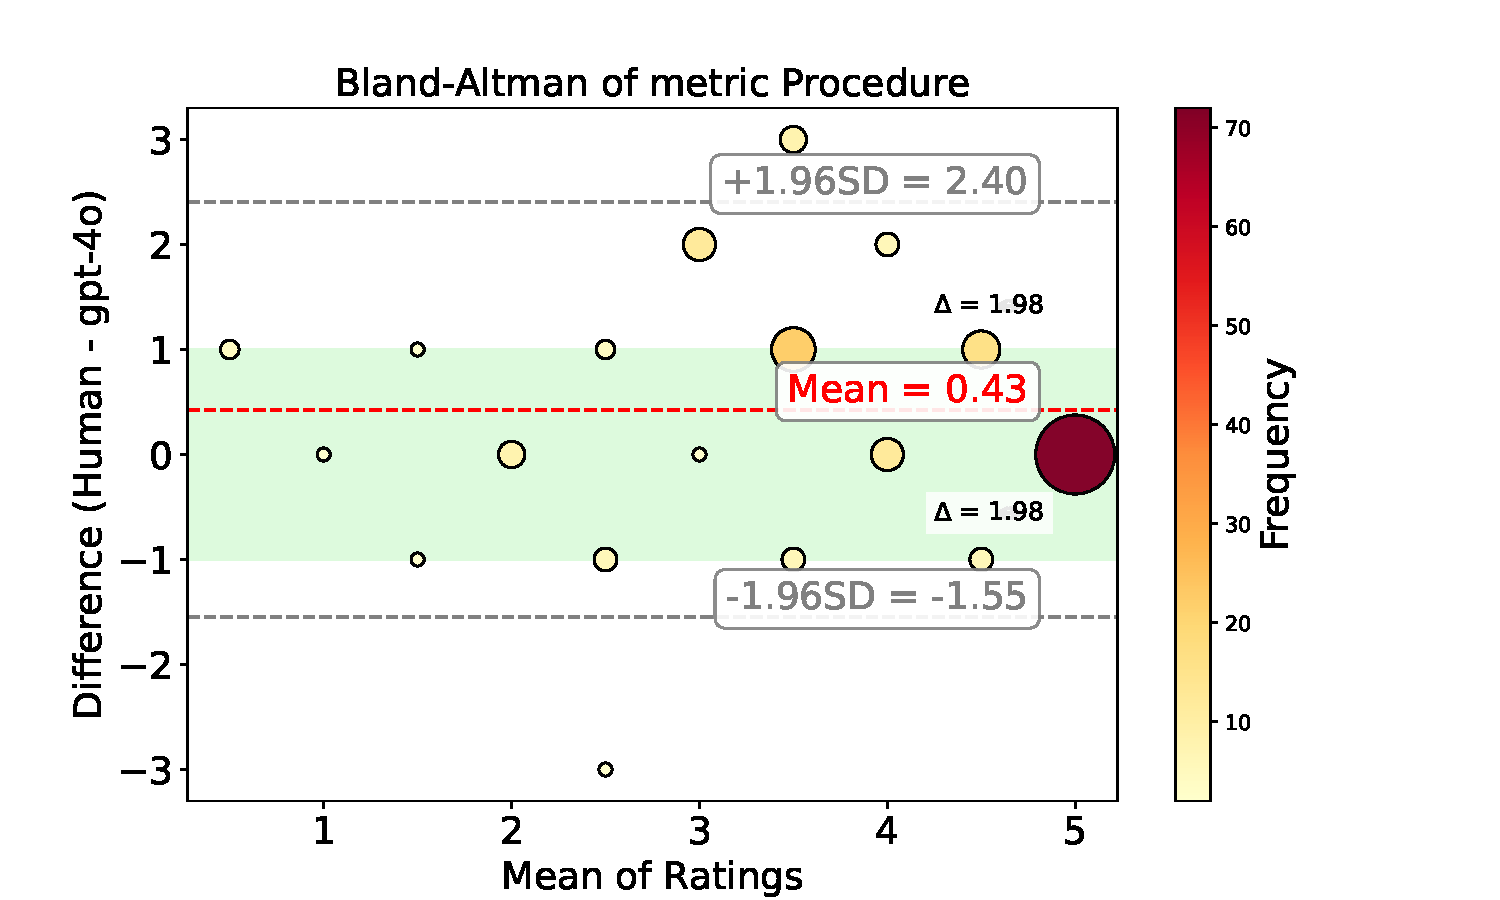
\includegraphics[width=\linewidth]{pic/Procedure_human_gpt-4o-2024-11-20.pdf}
        \caption{The Bland-Altman analysis result of \textbf{Procedure} with given key points.}
        \label{fig:w_keypointres_procedure}
    \end{minipage}
    \hfill % 添加一些水平间距
    \begin{minipage}[t]{0.48\textwidth}
        \centering
        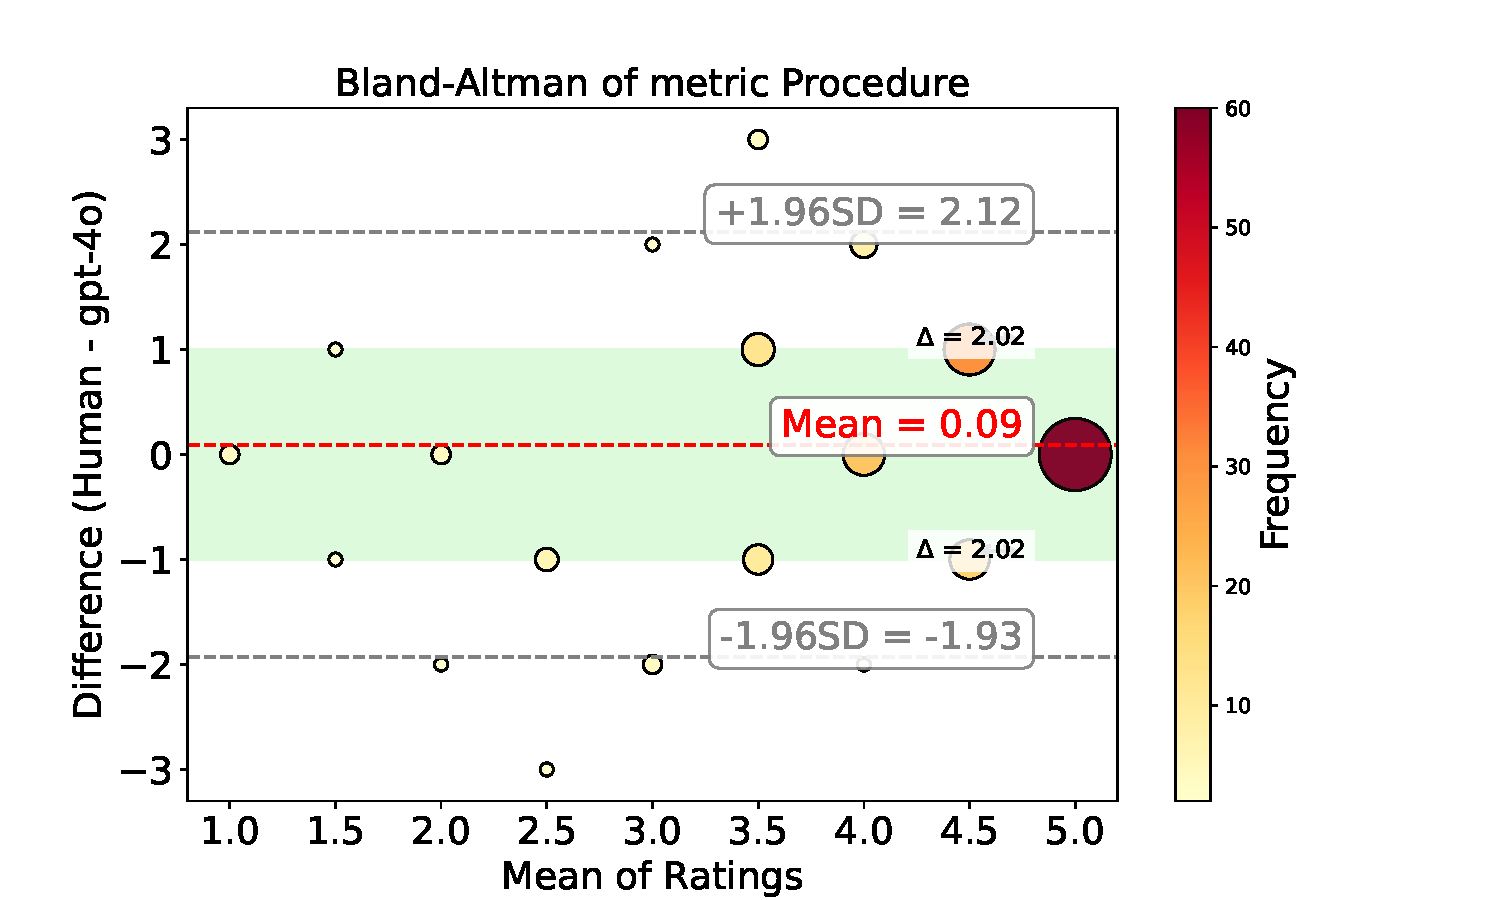
\includegraphics[width=\linewidth]{pic/Procedure_human_gpt-4o-2024-11-20_wk.pdf}
        \caption{The Bland-Altman analysis result of \textbf{Procedure} without given key points.}
        \label{fig:wo_keypoint_res_procedure}
    \end{minipage}
\end{figure*}

\begin{figure*}[htbp]
    \centering
    \begin{minipage}[t]{0.48\textwidth}
        \centering
        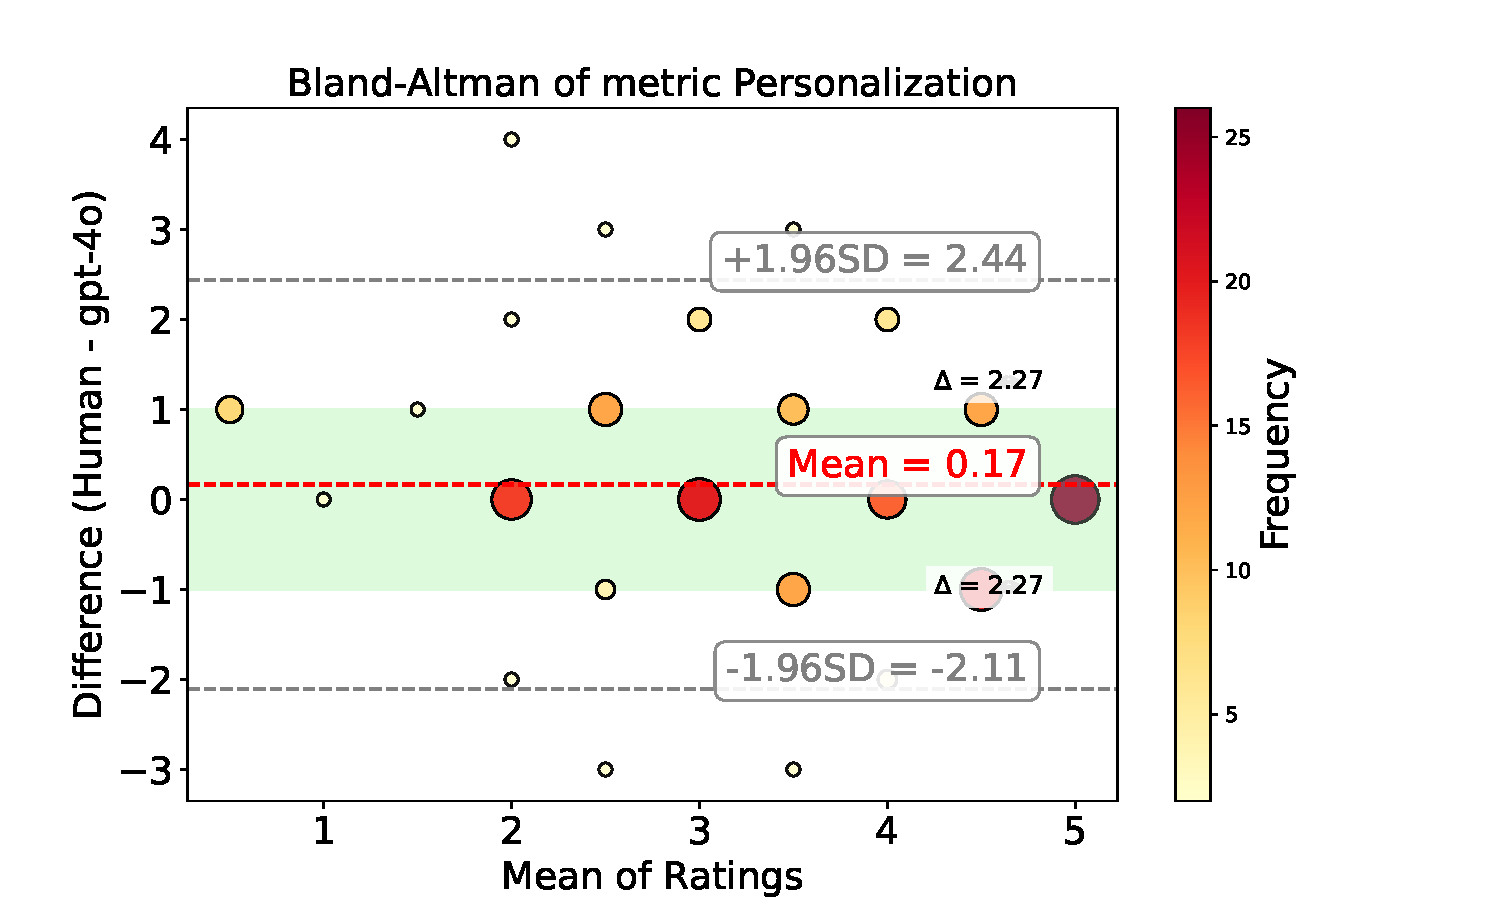
\includegraphics[width=\linewidth]{pic/Personalization_human_gpt-4o-2024-11-20.pdf}
        \caption{The Bland-Altman analysis result of \textbf{Personalization} with given key points.}
        \label{fig:w_keypoint_res_personalization}
    \end{minipage}
    \hfill % 添加一些水平间距
    \begin{minipage}[t]{0.48\textwidth}
        \centering
        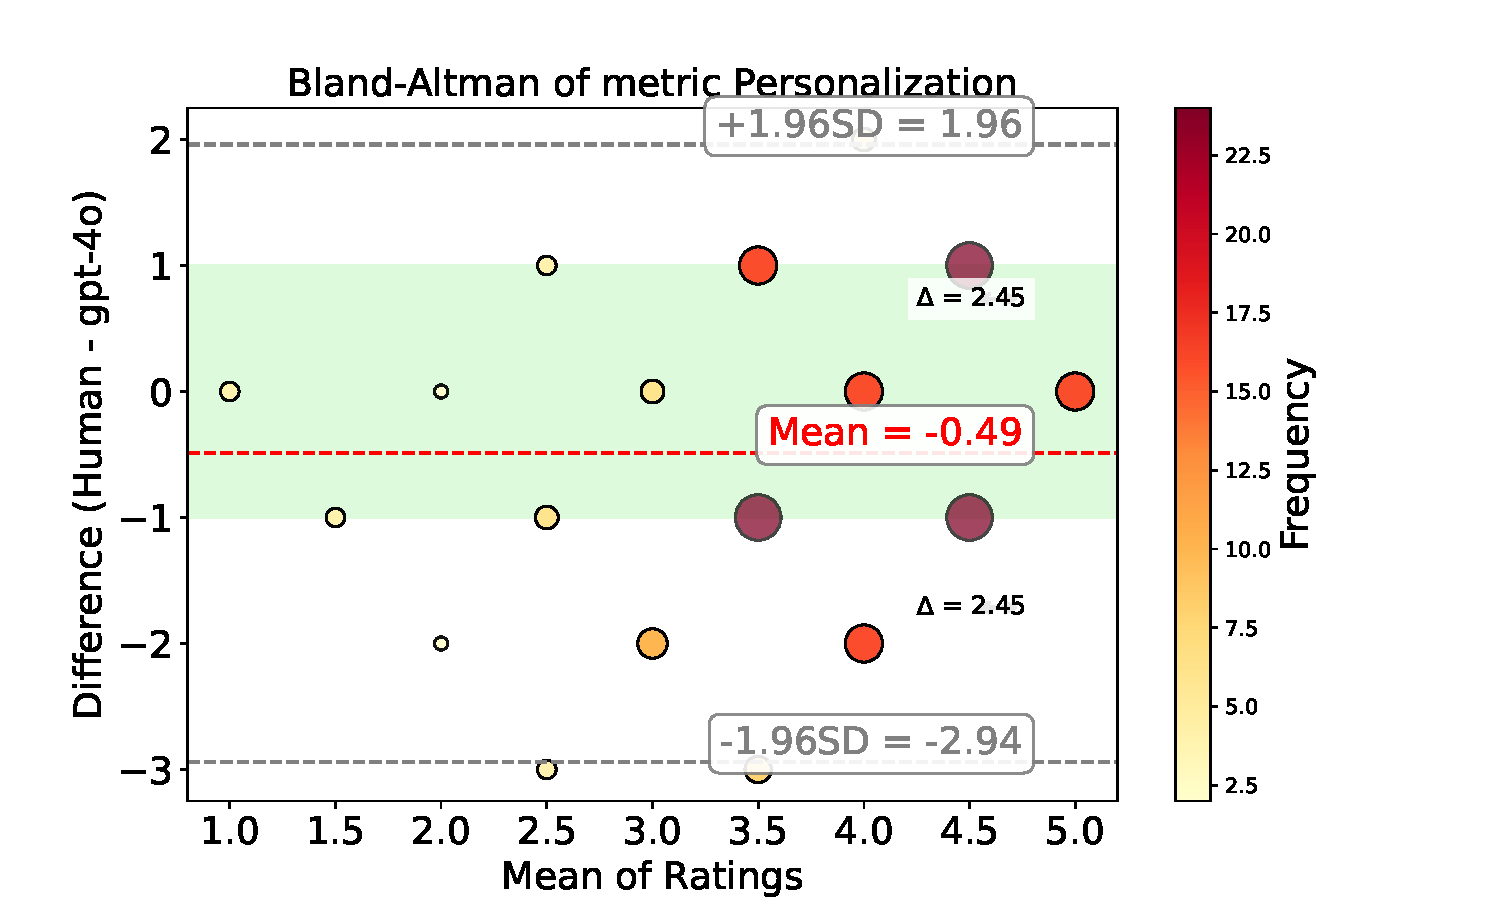
\includegraphics[width=\linewidth]{pic/Personalization_human_gpt-4o-2024-11-20_wk.pdf}
        \caption{The Bland-Altman analysis result of \textbf{Personalization} without given key points.}
        \label{fig:wo_keypoint_res_personalization}
    \end{minipage}
\end{figure*}






\newpage
\onecolumn
\begin{tcolorbox}[width=\textwidth, breakable]
{

\renewcommand{\lstlistingname}{Example}

\lstinputlisting[frame=none, basicstyle=\ttfamily\footnotesize, breaklines=true, columns=full, postbreak=\mbox{\textcolor{red}{$\hookrightarrow$}\space}, % Indicate line breaks% basicstyle=\ttfamily,    % Use monospaced font
    breakatwhitespace=true, label=Example:User_Profile, caption=User Profile Example, captionpos=b, ]{./profile.txt}
}




\end{tcolorbox}

\begin{tcolorbox}[width=\textwidth, breakable,]
{
\renewcommand{\lstlistingname}{Example}

\lstinputlisting[frame=none, basicstyle=\ttfamily\footnotesize, breaklines=true, columns=full, postbreak=\mbox{\textcolor{red}{$\hookrightarrow$}\space}, % Indicate line breaks% basicstyle=\ttfamily,    % Use monospaced font
    breakatwhitespace=true, label=Example:Tool_utilizing_Preference, caption=Tool-utilizing Preferences Example, captionpos=b, ]{./tool-utilizing_preference.txt}
}





\end{tcolorbox}

\begin{tcolorbox}[width=\textwidth, breakable, ]
{
\renewcommand{\lstlistingname}{Example}
% \label{Example:Interaction_History}
\lstinputlisting[frame=none, basicstyle=\ttfamily\footnotesize, breaklines=true, columns=full, postbreak=\mbox{\textcolor{red}{$\hookrightarrow$}\space}, % Indicate line breaks% basicstyle=\ttfamily,    % Use monospaced font
    breakatwhitespace=true, label=Example:Interaction_History, caption=Interaction History Example, captionpos=b, ]{./Interaction_History.txt}
}





\end{tcolorbox}
\begin{tcolorbox}[width=\textwidth, breakable, ]
{
\renewcommand{\lstlistingname}{Example}
% \label{Example:User_Profile}
\lstinputlisting[frame=none, basicstyle=\ttfamily\footnotesize, breaklines=true, columns=fullflexible, postbreak=\mbox{\textcolor{red}{$\hookrightarrow$}\space}, % Indicate line breaks% basicstyle=\ttfamily,    % Use monospaced font
    breakatwhitespace=true, label=Example:Example_of_Error, caption=Error Output Example, captionpos=b, ]{./Example_Error.txt}
}



\end{tcolorbox}



\newpage
% \onecolumn
\begin{tcolorbox}[width=\textwidth, breakable, ]
{
\renewcommand{\lstlistingname}{Prompt}
% \label{Prompt:ReAct_Tool_Given}
\lstinputlisting[frame=none, basicstyle=\ttfamily\footnotesize, breaklines=true, columns=fullflexible, postbreak=\mbox{\textcolor{red}{$\hookrightarrow$}\space}, % Indicate line breaks% basicstyle=\ttfamily,    % Use monospaced font
    breakatwhitespace=true, label=Prompt:ReAct_Tool_Given, caption=ReAct (Tool-Given), captionpos=b, ]{./Prompt_Template_ReAct_Tool_Given.txt}
}


\end{tcolorbox}



\begin{tcolorbox}[width=\textwidth, breakable, ]
{
\renewcommand{\lstlistingname}{Prompt}
% \label{Prompt:FC_Tool_Given}
\lstinputlisting[frame=none, basicstyle=\ttfamily\footnotesize, breaklines=true, columns=fullflexible, postbreak=\mbox{\textcolor{red}{$\hookrightarrow$}\space}, % Indicate line breaks% basicstyle=\ttfamily,    % Use monospaced font
    breakatwhitespace=true, label=Prompt:FC_Tool_Given, caption=FC (Tool-Given), captionpos=b,]{./Prompt_Template_FC_Tool_Given.txt}
}


\end{tcolorbox}

% \onecolumn
\begin{tcolorbox}[width=\textwidth, breakable, ]
{
\renewcommand{\lstlistingname}{Prompt}
% \label{Prompt:E-ReAct_Tool_Given}
\lstinputlisting[frame=none, basicstyle=\ttfamily\footnotesize, breaklines=true, columns=fullflexible, postbreak=\mbox{\textcolor{red}{$\hookrightarrow$}\space}, % Indicate line breaks% basicstyle=\ttfamily,    % Use monospaced font
    breakatwhitespace=true, label=Prompt:E-ReAct_Tool_Given, caption=E-ReAct (Tool-Given), captionpos=b,]{./Prompt_Template_E-ReAct_Tool_Given.txt}
}


\end{tcolorbox}


% \onecolumn
\begin{tcolorbox}[width=\textwidth, breakable, ]
{
\renewcommand{\lstlistingname}{Prompt}
% \label{Prompt:ReAct_Tool_Retrieval}
\lstinputlisting[frame=none, basicstyle=\ttfamily\footnotesize, breaklines=true, columns=fullflexible, postbreak=\mbox{\textcolor{red}{$\hookrightarrow$}\space}, % Indicate line breaks% basicstyle=\ttfamily,    % Use monospaced font
    breakatwhitespace=true, label=Prompt:ReAct_Tool_Retrieval, caption=ReAct (Tool-Retrieval), captionpos=b,]{./Prompt_Template_ReAct_Tool_Retrieval.txt}
}

\end{tcolorbox}


% \onecolumn
\begin{tcolorbox}[width=\textwidth, breakable, ] % (Tool-Retrieval)
{
\renewcommand{\lstlistingname}{Prompt}
% \label{Prompt:FC_Tool_Retrieval}
\lstinputlisting[frame=none, basicstyle=\ttfamily\footnotesize, breaklines=true, columns=fullflexible, postbreak=\mbox{\textcolor{red}{$\hookrightarrow$}\space}, % Indicate line breaks% basicstyle=\ttfamily,    % Use monospaced font
    breakatwhitespace=true, label=Prompt:FC_Tool_Retrieval, caption=FC (Tool-Retrieval), captionpos=b,]{./Prompt_Template_FC_Tool_Retrieval.txt}
}

\end{tcolorbox}


% \onecolumn
\begin{tcolorbox}[width=\textwidth, breakable, ]
{
\renewcommand{\lstlistingname}{Prompt}
% \label{Prompt:E-ReAct_Tool_Retrieval}
\lstinputlisting[frame=none, basicstyle=\ttfamily\footnotesize, breaklines=true, columns=fullflexible, postbreak=\mbox{\textcolor{red}{$\hookrightarrow$}\space}, % Indicate line breaks% basicstyle=\ttfamily,    % Use monospaced font
    breakatwhitespace=true, label=Prompt:E-ReAct_Tool_Retrieval, caption=E-ReAct (Tool-Retrieval), captionpos=b,]{./Prompt_Template_E-ReAct_Tool_Retrieval.txt}
}



\end{tcolorbox}


% \onecolumn
\begin{tcolorbox}[width=\textwidth, breakable, ]
{
\renewcommand{\lstlistingname}{Prompt}
% \label{Prompt:Key_Point_Evaluation}
\lstinputlisting[frame=none, basicstyle=\ttfamily\footnotesize, breaklines=true, columns=fullflexible, postbreak=\mbox{\textcolor{red}{$\hookrightarrow$}\space}, % Indicate line breaks% basicstyle=\ttfamily,    % Use monospaced font
    breakatwhitespace=true, label=Prompt:Key_Point_Evaluation, caption=Evaluation Prompt of key-point-based LLM Evaluation, captionpos=b,]{./Prompt_Evaluation.txt}
}



\end{tcolorbox}


% \onecolumn
\begin{tcolorbox}[width=\textwidth, breakable, ]
{
\renewcommand{\lstlistingname}{Example}
% \label{Example:Evaluation_Result_Example}
\lstinputlisting[frame=none, basicstyle=\ttfamily\footnotesize, breaklines=true, columns=full, postbreak=\mbox{\textcolor{red}{$\hookrightarrow$}\space}, % Indicate line breaks% basicstyle=\ttfamily,    % Use monospaced font
    breakatwhitespace=true, label=Example:Evaluation_Result_Example, caption=Evaluation Result Example, captionpos=b,]{./Evaluation_Result_Example.txt}
}



\end{tcolorbox}







\end{document}
